% !TEX root = ./../main.tex
\chapter{Introduction to Molecular Dynamics}
For macroscopic bodies, the motion of a system in time and space is governed by the classical equations of 
motion, say Newton’s laws, while reducing time and space scales, quantum mechanics kicks in. Despite the latter 
statement, classical laws of motion have proved to be a good approximation also at the molecular level, as long 
as atoms are massive enough.

In order to predict the time evolution of a complete system, such as the biomolecular system we will treat in 
this thesis, Newton’s equations of motion need to be integrated numerically. The necessity of a numerical 
integration arises from the complexity of the interactions involved in realistic systems, often nonlinear 
functions of positions and momenta of the particles, which makes it impossible to obtain an analytical solution 
for the equations of motion.

In the first part of this Chapter the laws of classical and statistical mechanics will be briefly summarized.
Then we will introduce the computational \acf{MD} method and analyze the main aspects of this technique with some 
details about the \textit{empirical} \ac{FF}: the container of system model and parameters under study. This 
includes the way to consider and treat the inter--particle interactions at \ac{MD} level. Then, coarse--graining 
procedure are introduced, with particular attention to the \martini \ac{FF}, the main \ac{FF} used in this thesis 
work. Lastly advanced sampling techniques are explained: the \textit{Umbrella Sampling} and 
\textit{Metadynamics}. This introductory Chapter are based on the books of Tuckerman \cite{Tuckerman}, Leach 
\cite{Leach}, Frenkel and Smit \cite{Frenkel} and Allen and Tildesley \cite{Allen} to which the reader is 
addressed for a more complete discussion.

\section{Review of classical mechanics}
Let us consider a system of $N$ particles with mass $m_i$ and coordinates $\vec r_1,\dots,\vec r_N$. According 
to the Newton's second low each particle will experience a total force $\vec F_i$ such that
\begin{equation}
	m_i \ddot{\vec{r}}_i = \vec F_i(\vec r_1,\dots,\vec r_N)
	\label{eq:newtonLaw}
\end{equation}
The total force on each particle is defined as
\begin{equation*}
	\vec F_i(\vec r_1,\dots,\vec r_N) = \vec{f}_i^{\ (e)}(\vec r_i) + \sum_{i\ne j}^N \vec{f}_{ij}^{\ (i)}(\vec r_i - \vec r_j )
\end{equation*}
where $\vec{f}_i^{\ (e)}$ is an external force acting on particle $i$ and $\vec{f}_{ij}^{\ (i)}$, which in general
depends only on distance between particle $i$ and $j$, is the inter-particle force that $i$ exerts on $j$ and
\textit{vice-versa}. Equations~\eqref{eq:newtonLaw} are refereed to as \textit{the equations of motion} of the
system; integrating them, with the sets of the \textit{initial conditions} at start time 
$t_0$ $\vec r_1(t_0),\dots,\vec r_N(t_0)$ and $\dot{\vec{r}}_1(t_0),\dots,\dot{\vec{r}}_N(t_0)$, the positions 
and the velocities of all the particles in the system at any time are known.

Another way to write the equations of motion is to use particles momenta $\vec p_i = m_i \dot{\vec{r}}_i$ and then
the equations~\eqref{eq:newtonLaw} become
\begin{equation}
	\frac{d\vec p_i}{dt} = \vec F_i(\vec r_1,\dots,\vec r_N)
	\label{eq:newtonLawMom}
\end{equation}
The full set of $6N$ functions $(\vec r_1(t),\dots,\vec r_N(t),\vec p_1(t),\dots,\vec p_N)$ gives us a full
description of the dynamics of the $N$--particle system. The set of functions above can be arranged in an ordered 
$6N$--dimensional vector
\begin{equation}
	\vec x(t) = (\vec r_1(t),\dots,\vec r_N(t),\vec p_1(t),\dots,\vec p_N)
	\label{eq:phSpaceVector}
\end{equation}
called \textit{phase space vector} or the \textit{microstate} of the system at time $t$. All the possible
microstates of a system generate a $6N$--dimensional space called \textit{phase space} of the system, indicated 
with $\Omega$. Thus $\vec x(t)$ describes a particular trajectory in the phase space, i.e. the system evolution 
is the motion of a phase space point. For simplicity of notation let us introduce also the ordered vectors $\vec r = (\vec r_1, \dots, \vec r_N)$, $\dot{\vec r} = (\dot{\vec{r}}_1,\dots,\dot{\vec{r}}_N)$ and $\vec p = (\vec p_1, \dots, \vec p_N)$ which are the coordinates, velocities and momenta off all particles.

Let us suppose that all the forces acting on the $N$--particle system are conservative; this means that it must
exist a scalar function $U = U(\vec r)$ called \ac{PEF}, such that
\begin{equation}
	\vec F(\vec r) = -\partial_{r_i} U(\vec r)\ \hat e_i = -\vec\nabla_{\vec r} U(\vec r)
	\label{eq:pefForces}
\end{equation}
where $\vec F = (\vec F_1,\dots, \vec F_N)$. Thus we have only to know the \ac{PEF} of the system at any time and 
the initial conditions to solve Newton's laws.

The kinetic energy of the system is defined as
\begin{equation}
	K(\dot{\vec r}) = \sum_{i=0}^{N}\frac{1}{2}m_i \dot{\vec r}_i\cdot \dot{\vec r}_i
	\label{eq:kinetic}
\end{equation}

If the system is conservative we can define a scalar function, called \textit{Lagrangian} of the system
\begin{equation}
	\mathcal{L}(\vec r,\dot{\vec r}) = K(\dot{\vec r}) - U(\vec r)
	\label{eq:lagrangian}
\end{equation}
such that
\begin{equation}
	\frac{d}{dt}\left ( \frac{\partial \mathcal{L}}{\partial \dot r_{i}}\right ) - \frac{\partial\mathcal{L}}{\partial r_{i}} = 0
	\label{eq:EulerLagrange}
\end{equation}
These set of $3N$ equations are called \textit{Euler--Lagrange equations of motion}. It is easy to show that 
substituting the definition of $\mathcal{L}$ we obtain the Newton's second law. The Euler--Lagrange equations are 
a sort of generator of the equations of motion.

Using the definition of $\mathcal{L}$ \eqref{eq:lagrangian} we have
\begin{equation}
	p_i = \frac{\partial\mathcal{L}}{\partial \dot r_i} = m_i\dot r_i
	\label{eq:momentaLagrangian}
\end{equation}
thus we can express particle velocities as a function of particle momenta. Equations~\eqref{eq:kinetic}
and~\eqref{eq:momentaLagrangian} let us to express the kinetic energy in the form
\begin{equation}
	K(\vec p) = \sum_{i=0}^N \frac{\vec p_i \cdot \vec p_i}{2m_i}
	\label{eq:kineticP}
\end{equation}

To describe the system we can define another scalar function, called \textit{Hamiltonian} of the system
\begin{equation*}
	\mathcal{H}(\vec r, \vec p) = \sum_{i=0}^N \vec p_i \cdot \dot{\vec r}_i(\vec p_i) - \mathcal{L}(\vec r, \dot{\vec r}(\vec p))
\end{equation*}
Substituting~\eqref{eq:lagrangian} and using~\eqref{eq:kineticP} the Hamiltonian of the system is nothing that
\begin{equation}
	\mathcal{H}(\vec r, \vec p) = K(\vec p) + U(\vec r)
	\label{eq:hamiltonian}
\end{equation}
or \textit{the total energy of the system}. To obtain the equations of motion we have to solve \textit{Hamilton's equations}
\begin{equation}
	\begin{aligned}
		\dot r_i &=& &\frac{\partial\mathcal{H}}{\partial p_{i}} \\
		\dot p_i &=&-&\frac{\partial\mathcal{H}}{\partial r_{i}}
	\end{aligned}
	\label{eq:eqhamilton}
\end{equation}
Describing the system with the Hamiltonian formalism, in some cases, is more useful than Lagrangian one, first of
all because the Hamiltonian of a system is directly related to a well know physical quantity, the total energy.

\section{Review of statistical mechanics}
\label{sec:statmec}
Using the picture of the classical mechanics described above we have a good and sophisticated machinery that 
allows us, knowing some information about the system in exam, i.e. initial positions and velocities of all 
particles and their interactions, to completely solve the equations of motion in order to get the dynamics of the 
system at every time. So classical mechanics encodes all the information about the \textit{microscopic} view of a 
system and, in principle, we can extract all the information we want about the \textit{macroscopic} proprieties 
of such system. The main task of this process is to obtain the thermodynamics proprieties of a system 
(temperature, pressure and so on) from the complete sets of positions and velocities of all particles and thus it 
is necessary to have a link between microscopic and macroscopic world.

The solution of that problem comes from \textit{statistical mechanics} developed, principally, by Boltzmann and 
Gibbs. Statistical mechanics involves all the rules and methods through which the microscopic and macroscopic 
worlds are related to each other. This provides also a rigorous derivation of thermodynamics from the microscopic 
proprieties: without that thermodynamics would be only a phenomenological theory. The first step to the solution 
of the problem is to recognize that \textit{a macroscopic observable of a system does not strongly depend on the 
complete dynamics of each particle in the system, but rather on an average that cancels out all the details of 
the microscopic features}. This it is intuitively true. We can think to set up an experiment with a system in a 
specific microscopic state that corresponds to a macroscopic state. Certainly we can do the contrary and for sure 
we wont find the same microscopic state. Then we can iterate the experiment and we will find that for a specific 
macroscopic state of a system there exists a number of microscopic states that yield to the same properties.

The most important concept that makes this idea practicable is the \textit{statistical ensemble}. Based on the 
previous considerations, a general definition of an ensemble is \textit{a collection of systems subject to a set 
of common interactions and sharing the same macroscopic properties}. This concept lays the foundations of 
thermodynamics and suggests a procedure to compute many macroscopic observables. In more details a 
$N$--particle system in a specific microscopic state is described by its microstate $\vec x$, then \textit{an 
ensemble is a set of points in the phase space that are subject to the constraint to be part of the ensemble 
itself}. Each system evolves in time with the equations of motion, so the time evolution of an ensemble is 
described by the flow of a set of points in the phase space according to the classical mechanics.

Once an ensemble is defined we are able to compute, at every time, the macroscopic observables simply averaging 
over all systems in the ensemble. To do this we have to know, at every time, which microstates of the phase space 
are part of the ensemble. For this purpose we define the \textit{ensemble distribution function} 
$\tilde\rho = \tilde\rho(\vec x,t)$. Let $dx = dr_1\cdots dr_{3N} dp_1 \cdots dp_{3N}$ the infinitesimal phase 
space volume, then
\begin{equation*}
	\frac{1}{\mathcal{N}}\tilde\rho(\vec x, t)\ dx = \rho(\vec x, t)\ dx ????
\end{equation*}
where $\mathcal{N}$ is the total number of microstates in the ensemble. $\rho(\vec x, t)dx$ can be interpreted as 
the probability to find in the ensemble a system with microstate $\vec x$ at a time $t$ and $\rho(\vec x, t)$ is 
the more convenient normalized distribution function. For definition of probability density must be
\begin{equation*}
	\int_{\Omega} \rho(\vec x, t)\ dx = 1, \qquad \rho(\vec x, t) \ge 0
\end{equation*}

Giving the ensemble distribution function, the ensemble average of an observable $A=A(\vec x)$, at every time, is 
defined as
\begin{equation*}
	\ave{A}(t) = \int_\Omega A(\vec x)\rho(\vec x, t)\ dx
\end{equation*}
For an ensemble at thermodynamic equilibrium the macroscopic state is fixed and so, if $A$ is an equilibrium 
observable, it must be time--independent. Thus, it can be shown \cite{Tuckerman} that exist a scalar function of 
the Hamiltonian $\mathit{f}(\mathcal{H}(\vec x))$ such that the time--independent ensemble average of the 
equilibrium observable $A$ can be expressed as 
\begin{equation*}
	\ave{A} = \frac{1}{\mathcal{Z}} \int_\Omega A(\vec x, t) \mathit{f}(\mathcal{H}(\vec x))\ dx
\end{equation*}
where $\mathcal{Z}$, known as \textit{partition function}, is specific for the ensemble in exam and it is defined 
as follow
\begin{equation*}
	\mathcal{Z} = \int_\Omega \mathit{f}(\mathcal{H}(\vec x))\ dx
\end{equation*}

In order to compute the partition function we need to specify the thermodynamic observables, called 
\textit{control variables}, that characterize the ensemble itself. By definition of an ensemble at thermodynamic 
equilibrium those control variables must be constant in time. The main ensembles used in statistical mechanics 
and the related control variables are summarized as follow
\begin{itemize}
	\item \textit{microcanonical ensemble}: constant--$NVE$
	\item \textit{canonical ensemble}: constant--$NVT$
	\item \textit{isothermal--isobaric ensemble}: constant--$NpT$
	\item \textit{grand--canonical ensemble}: constant--$\mu pT$
\end{itemize}
The averages computed in different ensembles are equivalent in the so called \textit{thermodynamic limit}: this 
is the \textit{equivalence of ensembles}. Thus, it must be possible to change from one ensemble to another 
leaving averages unchanged.

We have defined ensemble averages and how to compute them but we need also a link between statistical averages 
and the experimental values. When we measure a macroscopic observable $A$ we prepare an experiment with 
\textit{only one} system in a specific macroscopic state and we study its evolution in time. $A$ is a function of 
time and phase space vector and it fluctuates over time due to particle interactions. The measurement itself 
requires long time intervals compared to microscopic time scales, thus when we measure an observable we take an 
\textit{average over time}. If, in principle, the time for average is infinity then we have the ``real'' mean 
value of the observable
\begin{equation*}
	\overline{A} = \lim_{\tau\to +\infty}\frac{1}{\tau}\int_{t_0}^\tau A(\vec x_t)\ dt
\end{equation*}
In order for a comparison to be made, an identity between ensemble and time averages must be established.
This link is provided by the \textit{ergodic theorem} and the \textit{ergodic hypothesis}. A system is said to be 
ergodic if, over a long period of time, all the microstates in the phase space with the same energy are 
accessible with the same probability. Then the ergodic theorem says that, if the system is ergodic, the time and 
ensemble averages are equal \textit{almost everywhere} in the phase space. So we can write the follow identity
\begin{equation}
	\overline{A} = \lim_{\tau\to +\infty}\frac{1}{\tau}\int_{t_0}^\tau A(\vec x(t))\ dt = \int_\Omega A(\vec x)\rho(\vec x, t)\ dx = \ave{A}(t)
	\label{eq:ergotic}
\end{equation}

For biomolecular applications the most important ensembles are the microcanonical and the isothermal--isobaric. 
In the following we will describe them briefly with particular attention to the isothermal--isobaric ensemble, 
the most relevant for this thesis work.

\subsection{Microcanonical ensemble}
The microcanonical ensemble is composed of the systems whose number of particles ($N$), volume ($V$) and energy 
($E$) are constant. Due to the constant energy it describes a Hamiltonian system for which
\begin{equation*}
	\mathcal{H}(\vec x) = E
\end{equation*}
this let us to define the partition function as follow
\begin{equation}
	\mathcal{Z}_{NVE} = \frac{1}{N!h^{3N}}\int_\Omega \delta(\mathcal{H}(\vec x) - E)\ dx
	\label{eq:micropartition}
\end{equation}
where the normalization factor $N!$ takes into account the particles indistinguishability and $h^{3N}$ is for 
compatibility of statistical mechanics with quantum mechanics: it comes from Heisenberg’s uncertainty principle 
and it is the smallest phase space volume element. The right thermodynamic potential, i.e. the constant of 
motion, to obtain all the macroscopic observables is the entropy $S$ given by
\begin{equation*}
	S = k_B \ln \mathcal{Z}_{NVE}
\end{equation*}
where $k_B = 1.3806505(24) \cdot 10^{-23}$~J/K is the Boltzmann constant. The other thermodynamic quantities can 
be obtained by
\begin{equation*}
	\frac{1}{T} = \left ( \frac{\partial S}{\partial E}\right )_{NV} \qquad \frac{p}{T} = \left ( \frac{\partial S}{\partial V}\right )_{NE} \qquad \frac{\mu}{T} = \left ( \frac{\partial S}{\partial N}\right )_{VE}
\end{equation*}

The link between microscopic functions of phase space points and macroscopic observables, like kinetic energy or 
pressure, is provided by the \textit{classical virial theorem} which states that
\begin{equation}
	\ave{x_i\frac{\partial\mathcal{H}}{\partial x_k}} = k_B T \delta_{ik}
	\label{eq:virial}
\end{equation}
where $x_i$ is some phase space variable.
% often the virial theorem is written in a slightly different form
% \begin{equation}
% 	\ave{K} = - \frac{1}{2}\sum_{i=1}^{3N} \ave{F_ir_i}
% \end{equation}
% where $\ave{K}$ is the average kinetic energy, not necessary at equilibrium and $F_i$ is the total forces acting on particle $i$. Both are valid even if the system is not at the equilibrium.

\paragraph{\textbf{Kinetic energy}} Since a system in a microcanonical ensemble is defined to be Hamiltonian, 
from equations~\eqref{eq:hamiltonian} and~\eqref{eq:kineticP} according to the virial theorem with the choice 
$x_i = p_{i}$ we obtain
\begin{equation*}
	\ave{\frac{p^2_{i}}{m_i}} = k_bT
\end{equation*}
then summing both side over all particles and over the three coordinates we obtain the average kinetic energy at 
equilibrium
\begin{equation}
	\ave{K} = \ave{ \sum_{i=1}^{N}\sum_{\alpha=1}^{3}\frac{p_{i+\alpha}^2}{2m_i} } = \ave{\sum_{i=1}^{N}\frac{\vec p_i\cdot \vec p_i}{2m_i}} = \frac{3}{2}Nk_B T
	\label{eq:kineticT}
\end{equation}
this is like the well know equipartition theorem in which $3N$ is the number of \ac{DOF}.

\paragraph{\textbf{Pressure}} Choosing $x_i = r_i$ in equation~\eqref{eq:virial} and summing both side over all particles and substituting equations~\eqref{eq:eqhamilton} and~\eqref{eq:kineticT}, we obtain
\begin{equation*}
	W = \ave{\sum_{i=1}^{3N} r_i\dot p_i} = -3Nk_B T = - 2 \ave{K}
\end{equation*}
the quantity $W$ is often called \textit{virial}. For a $N$--particle non--interacting system it is well known 
that $pV = Nk_B T$ thus the virial is $W = -3pV$. For a real interacting system we need to include in the virial 
the contribution due to the inter--particles interactions $U(\vec r_1,\dots,\vec r_N)$, thus the virial 
becomes\footnote{We assume that the inter--particles interactions are pairwise addictive which they depends only 
on distances between particles $i$ and $j$.}
\begin{equation*}
	W = -3pV + \ave{ \sum_{i=1}^N\sum_{j=i+1}^Nr_{ij}f_{ij} } = - 2 \ave{K}
\end{equation*}
where $r_{ij}$ and $f_{ij}$ are the distance and force between particles $i$ and $j$. Thus the pressure of the 
system is given by
\begin{equation*}
	p = \frac{1}{3V}\left (2 \ave{K} + \ave{ \sum_{i=1}^N\sum_{j=i+1}^Nr_{ij}f_{ij} } \right )	
\end{equation*}
The instantaneous pressure in terms of the phase space points $\vec x(t)$ is obtained substituting 
equation~\eqref{eq:kineticT} and getting the quantity in the average bracket, so
\begin{equation}
	p(\vec x_t) = \frac{1}{3V} \sum_{i=1}^{N} \left ( \frac{\vec p_i \cdot \vec p_i}{m_i} +  \sum_{j=i+1}^Nr_{ij}f_{ij}  \right )
	\label{eq:pressure}
\end{equation}

\subsection{Isothermal--isobaric ensemble}
The isothermal--isobaric ensemble contains those systems with constant particles number ($N$), pressure ($p$) and 
temperature ($T$). This is useful in many chemical, biological and physical systems since their properties are 
reported in conditions of standard temperature and pressure. To maintain the system at constant temperature and 
pressure it is necessary to couple it with an external \textit{temperature bath} and a \textit{pressure bath}. 
The first one can be considered simply a very big system at constant temperature with a high thermal capacity. 
The second can be idealized like a piston connected to the system: it change the volume in order to adjust the 
pressure. The instantaneous work done by the system against the external piston is defined by $pV$, where $V$ is 
the instantaneous system volume. Then we have to correct the Hamiltonian of the system: 
$\mathcal{H}(\vec x) \rightarrow \mathcal{H}(\vec x) + pV$. The partition function is then defined considering 
the Boltzmann ensemble distribution function
\begin{equation}
	\mathcal{Z}_{NPT} = \frac{1}{N!h^{3N}}\int_0^{+\infty}\ dV \ \int_\Omega e^{-\beta(\mathcal{H}(\vec x) + pV)}\ dx
	\label{eq:nptPartition}
\end{equation}
where $\beta^{-1} \equiv k_B T$ and the normalization factor is the same as in 
equation~\eqref{eq:micropartition}. The right thermodynamic potential, i.e. the constant of motion, to obtain the 
other thermodynamic quantities is the Gibbs free energy $G = H - TS$ (where $H$ is the enthalpy) defined by
\begin{equation*}
	G = -k_B T\ln \mathcal{Z}_{NpT}
\end{equation*}
it describes the maximum reversible work that may be performed by the system. The other thermodynamic quantities 
can be obtained by
\begin{equation*}
	\mu = \left ( \frac{\partial G}{\partial N}\right )_{pT} \qquad \ave{V} = \left ( \frac{\partial G}{\partial p}\right )_{NT} \qquad S = \left ( \frac{\partial G}{\partial T}\right )_{Np}
\end{equation*}

For anisotropic systems, volume can undergo different changes in the three Cartesian directories even if external 
pressure is applied isotropically. In these cases it is necessary to take this into account in the partition 
function. The way is to define a matrix formed by the three basis vectors of the system box $\vec a$, $\vec b$ 
and $\vec c$
\begin{equation}
	 \mathbold{H} = 
	\begin{pmatrix}
		a_1 & b_1 & c_1 \\
		a_2 & b_2 & c_2 \\
		a_3 & b_3 & c_3 \\
	\end{pmatrix}
	\label{eq:volumeMatrix}
\end{equation}
so that its volume is $V = \vec a\cdot \vec b\times \vec c = |\det{ \mathbold{H}}|$. The partition function become
\begin{equation*}
	Z_{NpT} = \frac{1}{N!h^{3N}}\int\ d \mathbold{H} \ \int_\Omega \frac{1}{(\det{H})^2} e^{-\beta(\mathcal{H}(\vec x) + p|\det{ \mathbold{H}}|)}\ dx
\end{equation*}
where $\int\ d\mathbold{H}$ is an integral over all nine components of $\mathbold{H}$. Hence, the instantaneous 
pressure can no longer be described by a single quantity. Instead a $3\times 3$ pressure matrix $ \mathbold{P}$ 
is needed. What one find, if the system is isotropically coupled, is that on average, this pressure matrix 
reduces to a diagonal pressure matrix such that
\begin{equation*}
	\text{Tr}\ave{ \mathbold{P}} = 3p
\end{equation*}

%eventualmente vedere se mettere le fluttuazioeni di energia e volume

\section{Molecular Dynamics simulation}
\label{sec:MD}
\acf{MD} is a set of techniques that allow us to prepare a ``computer experiments'' in which solving numerically 
the classical equations of motion of a virtual system we will be able to know its time evolution. Such virtual 
experiment approach has the advantage that many experiments can be set up with different initial conditions 
and/or with different control parameters, such as temperature or pressure. Obviously that experiment is carried 
out using a model that approximates the real system. The main parts of that model are the information required to 
obtain an approximation of the interactions among all system particles, i.e. to compute the \ac{PEF} from which 
the forces are derived by equation~\eqref{eq:pefForces}. Solving the equations of motion with a numerical 
integrator, an \ac{MD} simulation generates a set of phase space vectors, a \textit{trajectory}, at discrete 
times that are multiples of the fundamental time discretization parameter, called \textit{MD time step}; 
$\delta t$. Starting from an initial phase space vector $\vec x(0)$, at each step, the forces are computed from 
the \ac{PEF}. Then the equations of motion are integrated and a new phase space vector $\vec x(\delta t)$ is 
generated, thus a new set of forces is computed and so on. In order to compute time averages we need to 
discretize equation~\eqref{eq:ergotic} so the time integration is substituted with a summation over the collected 
data at certain time step $\Delta \tau = i \delta t$, $i=1,2,3,\dots$. If $i > 1$ only a subset of the collected 
data is used to compute time averages. The formula becomes
\begin{equation}
	\ave{A} = \frac{1}{M}\sum_{n=1}^M A(\vec x(n\Delta \tau))
	\label{eq:MDTimeAve}
\end{equation}
where $M\Delta \tau$ is the total averaged time and of course it must be $M \le D/i$ if $D$ is the total number 
of \ac{MD} steps. An \ac{MD} simulation can be summarized in the scheme in figure~(\ref{fig:MDscheme}).
\begin{figure}[!ht]
\centering
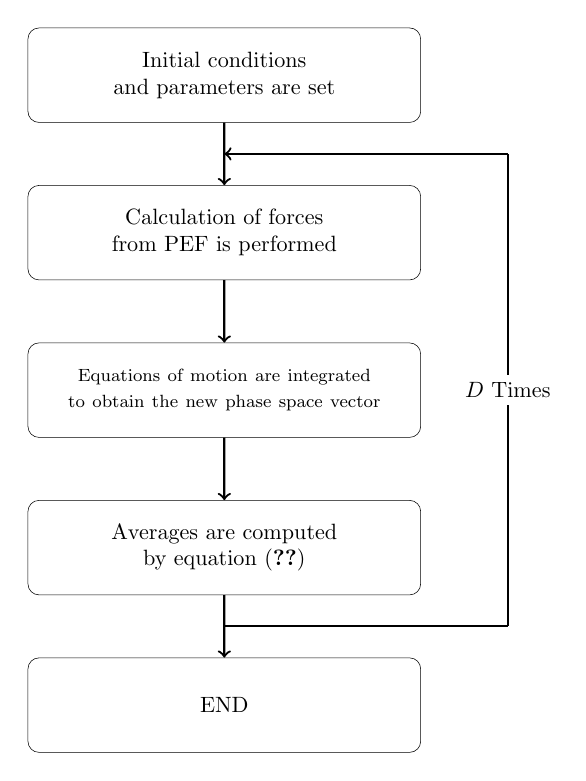
\begin{tikzpicture}[scale=0.8, transform shape]
	\node[rectangle,draw,rounded corners,very thin,minimum width=6cm,minimum height=1.5cm,text width=6cm,align=center] (A) at (0,10) {Initial conditions \\ and parameters are set};
	\node[rectangle,draw,rounded corners,very thin,minimum width=6cm,minimum height=1.5cm,text width=6cm,align=center] (B)  at (0,7.5) {Calculation of forces \\ from \ac{PEF} is performed};
	\node[rectangle,draw,rounded corners,very thin,minimum width=6cm,minimum height=1.5cm,text width=6cm,align=center] (C)  at (0,5) {\footnotesize Equations of motion are integrated to obtain the new phase space vector};
	\node[rectangle,draw,rounded corners,very thin,minimum width=6cm,minimum height=1.5cm,text width=6cm,align=center] (D)  at (0,2.5) {Averages are computed \\ by equation~(\ref{eq:MDTimeAve})};
	\node[rectangle,draw,rounded corners,very thin,minimum width=6cm,minimum height=1.5cm,text width=6cm,align=center] (E)  at (0,0) {END};
	\draw[thick,->] (A) -- (B);
	\draw[thick,->] (B) -- (C);
	\draw[thick,->] (C) -- (D);
	\draw[thick,->] (D) -- (E);
	\draw[thick,-] (0,1.25) -- (4.5,1.25);
	\draw[thick,-] (4.5,1.25) -- (4.5, 8.75) node[pos=0.5, fill=white] {$D$ Times};
	\draw[thick,->] (4.5, 8.75) -- (0, 8.75);
\end{tikzpicture}
\caption{Schematic representation of an \acs{MD} simulation.}
\label{fig:MDscheme}
\end{figure}

\subsection{Initial configuration}
Before an \ac{MD} simulation can be performed it is necessary to select an \textit{initial configuration}. Its 
choice can be nontrivial and it depends on the complexity of the system. Then, careful attention must be paid in 
setting up the initial configuration.

Setting up an initial configuration means to prepare an $N$--particle system and assign all particle positions 
and velocities, i.e. all the $6N$ coordinates of the initial phase space vector $\vec x(0)$. A common choice to 
assign the initial velocities is to extract they randomly from the Maxwell--Boltzmann distribution function at a 
specific system's temperature
\begin{equation*}
	f(v_i) = \sqrt{\frac{m_i}{2\pi k_B T}}e^{-\left ( \frac{m_iv_i^2}{2k_B T}\right )}
\end{equation*}
Moreover, the random assignment algorithm has to rescale all the velocities in such a way that the total system's 
momentum $\vec P = \sum_{k=1}^N m_k\vec v_k$ is zero, this is equivalent to a \ac{COM} motion removal. This is 
done because, in general, the total force acting on the system $\vec F = \sum_{k=1}^N \vec F_i$ is zero, then the 
\ac{COM} motion is constant and to avoid a constant drift of the system in space this can be removed. Of course 
this is a constraint on the system and it must be taken into account because it reduces the system \ac{DOF} by three.

\subsection{Periodic boundary conditions}
In an \ac{MD} simulation the sample system is inserted into a \textit{simulation box} whose shape can be 
differently chosen to better reproduce the symmetry of the simulated system. That box gives us the trivial 
possibility to introduce a well defined reference system of coordinates. Obviously we must not forget to 
correctly treat the \textit{boundary conditions}. In order to avoid surface effects and to consider only an 
infinite bulk system, \ac{PBC} are imposed to the simulation box. This gives us also the possibility to simulate 
system's bulk proprieties without considering a too large number of particles.
\begin{SCfigure}
	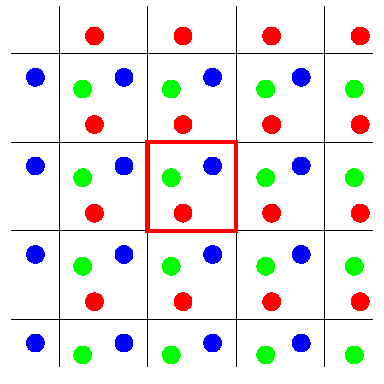
\includegraphics[width=0.5\textwidth]{./img/PBCScheme/PBCScheme}
	\caption{Schematic view of a two--dimensional box with \acs{PBC} imposed. The central, red contoured, box is the simulation box and it is replicated along each side.}
	\label{fig:pbc}
\end{SCfigure}
To give a better idea, in figure~(\ref{fig:pbc}) an example of a two--dimensional box with \ac{PBC} is shown. The 
central red contoured box is the simulation box. The idea is to replicate that box in space along each side so 
that there are no surface particles nor walls in the central box. When a particle moves in the central box, all 
its images virtually move the same way in the copies of the box so that if a particle leaves the virtual boundary 
of the central box, then, its nearest image enters the box and the number density of particles in the simulation 
box is conserved. This virtual movement of image particles is achieved adjusting the positions of the simulation 
box particles which have left the main box. For example, if one use a cubic box and a particle crosses its 
boundary in one direction, say the $x$ direction, then its coordinate is corrected by subtracting (if it leaves 
the box in the positive direction) or adding the box side length parallel to $x$ direction. Only box geometries 
compatible with translational symmetry can be used. For example, nether a spherical nor a icosahedral box could 
do the job. However when it is possible one have to use the most appropriate shape to better describe the 
symmetry of the system, otherwise a closest approximation, compatible with \ac{PBC}, must be used.

Even if \ac{PBC} are used in a wide range of applications, it must be taken into account that imposing 
periodicity to a system may affect its properties. A clear limitation of the periodic cell is that it is not 
possible to achieve fluctuations that have a wavelength greater then the cell length. This cause, obviously, the 
impossibility to sample those vibrating modes. Another problem arises with the range of the inter--particles 
interactions: one have to choose carefully the size of the simulation box, or the number of particles if an $NPT$ 
ensemble is used, to ensure that the smallest simulation box length is greater then the interaction range. This 
can be made easily for example with the Van der Waals interaction. On the contrary it is a difficult and time 
consuming task to do the same with the electrostatic interactions that are treated with a more sophisticated 
methods, as better explained in section~\ref{sec:longRangeInt}.

\subsection{Numerical integrators}
As we have seen above we need to solve numerically the equations of motion. Since the \ac{PEF} is a continuous 
function of the phase space vector at a time $t$, the simplest way is to use the so called \textit{finite 
difference} method. The basic idea is to expand the Newton's law in a Taylor series as follow
\begin{equation}
	\vec r_i(t + \delta t) = \vec r_i(t) + \vec v_i(t)\ \delta t + \frac{1}{2m_i}\vec f_i(t)\ (\delta t)^2\ +\ o((\delta t)^3)
	\label{eq:newtonTaylor}
\end{equation}
where we used the identities $\vec v_i(t) = \dot{\vec r}_i(t)$ and $m_i\ddot{\vec r}_i(t) = \vec f_i(t)$.

From this point, different algorithms have been developed. In the following we will describe in detail the most 
important, the \textit{Verlet algorithm}, and its implementation the \textit{leap--frog algorithm}, which is the 
default used in our \ac{MD} tools for this thesis work.

\subsubsection{Verlet algorithm}
The Verlet algorithm requires the positions and the forces at a time $t$ and the positions at a time $t-\delta t$ 
to calculate the positions at a time $t+\delta t$. Starting from equation~\eqref{eq:newtonTaylor} we can write
\begin{align}
	\vec r_i(t+\delta t) &\simeq \vec r_i(t) + \vec v_i(t)\delta t + \frac{1}{2m_i}\vec f_i(t)\ (\delta t)^2
	\label{eq:verlet1} \\
	\vec r_i(t-\delta t) &\simeq \vec r_i(t) - \vec v_i(t)\delta t + \frac{1}{2m_i}\vec f_i(t)\ (\delta t)^2
	\label{eq:verlet2}
\end{align}
from their sum we obtain the new positions at a time $t+\delta t$
\begin{equation}
	\vec r_i(t+\delta t) \simeq 2 \vec r_i(t) - \vec r_i (t - \delta t) + \frac{1}{m_i}\vec f_i(t)\ (\delta t)^2
	\label{eq:verletPosition}
\end{equation}
The velocities do not appear in the equation above and can be obtained taking the difference of 
equation~\eqref{eq:verlet1} and~\eqref{eq:verlet2}
\begin{equation*}
	\vec v_i(t) \simeq \frac{\vec r_i(t+\delta t) - \vec r_i(t-\delta t)}{2\delta t}
\end{equation*}

Since positions in equation~\eqref{eq:verletPosition} are computed as differences this is a fourth order 
algorithm and the precision is up to $o(\delta t)^4$, but they also contain a small term of order 
$o(\delta t)^2$, ($\vec f_i(t)/(2m_i)$) which is summed to a difference of larger terms 
($2 \vec r_i(t) - \vec r_i (t - \delta t)$). This may cause a loss of precision due to computer numerical representation.

The main disadvantage is that velocities at a time $t$ are an output of the calculation and not a part of the 
algorithm itself. Moreover it is not self--starting because the algorithm required the positions at a time 
$t-\delta t$. So at $t=0$ we need a trick to obtain the previous inexistent positions. The trick is to use 
equation~\eqref{eq:verlet2} truncated at the first order: $\vec r_i(-\delta t) \simeq \vec r(0) - \vec v_i(0)\delta t$.

\subsubsection{Leap--Frog algorithm}
The leap--frog algorithm is a variant of the Verlet one and it is commonly implemented in many \ac{MD} tools, as 
it is in our case. It computes the positions at a time $t$ and the velocities at a time 
$t+\nicefrac{1}{2}\delta t$ from the forces at a time $t$ and the velocities at a time 
$t-\nicefrac{1}{2}\delta t$. The main advantage with respect to the Verlet algorithm, is that it is 
self--starting because it does not require the positions at a time $t-\delta t$.

First it calculates the velocities at a time $t+\nicefrac{1}{2}\delta t$ as follow
\begin{equation*}
	\vec v_i(t + \nicefrac{1}{2}\delta t) \simeq \vec v_i(t - \nicefrac{1}{2}\delta t) + \vec a_i(t)\delta t
\end{equation*}
then the positions at a time $t+\delta t$ are computed
\begin{equation*}
	\vec r_i(t + \delta t) \simeq \vec r_i(t) + \vec v_i(t + \nicefrac{1}{2}\delta t)\delta t
\end{equation*}
The velocities at a time $t$ can be calculated by
\begin{equation}
	\vec v_i(t) \simeq \frac{\vec v_i(t + \nicefrac{1}{2}\delta t) + \vec v_i(t - \nicefrac{1}{2}\delta t)}{2}
	\label{eq:lfVelocitiesSync}
\end{equation}

Another advantage is that the velocities are part of the algorithm itself and moreover it does not require the 
calculation of the difference between two large numbers, with a gain of precision. The obvious disadvantage is 
that the positions and velocities are not synchronized so the equation~\eqref{eq:lfVelocitiesSync} is necessary 
to calculate the velocities at a time $t$. The need to have velocities at the same time of positions, as for the 
Verlet algorithm, derives from the calculation of the kinetic energy contribution to the total energy: it must be 
computed with positions and velocities at the same time.
%Discorso energia cinetica nello stesso tempo delle posizioni

\subsection{Neighbor list}
\label{sec:neighbor}
In order to solve the classical equations of motion, it is necessary to know the forces, and so the \ac{PEF}, 
acting on the system's particles. As we shall see in detail in the next section, this is one of the most time 
consuming part of an \ac{MD} simulation. To know the forces acting on one particle, in principle, it is necessary 
to calculate the contribution from all particles in the simulation box and all other periodic images. The most 
popular way to speed up the simulation is to use a truncation of the interaction potentials within a cutoff. The 
general idea is to compute the energy contribution of particle $i$ considering the interaction only with 
particles $j$ that are closer to a certain cutoff distance $r_c$, thus such that 
$\|\vec r_i - \vec r_j\| \le r_c$. This is summarized in the following expressions
\begin{equation*}
	U_i(\vec r) = \sum_{j\ne i}^N U^*_{ij}(\vec r), \qquad U^*_{ij}(\vec r) = \left \{
	\begin{aligned}
		& U_{ij}(\vec r)& \qquad  &\| \vec r_i - \vec r_j \| \le r_c \\
		& 0			    & \qquad  &\text{otherwise}
	\end{aligned}
	\right .
\end{equation*}
where $U_{ij}(\vec r)$ is the interaction potential between particles $i$ and $j$.

By itself, the use of a truncation of the potential may not dramatically reduce the time spent in computing the 
inter--particle interactions. This is because, in order to decide for what particles we have to compute the 
interactions, we have to compute the distances between every pair of particles in the system. A marked increase 
of performance is achieved by the use of a \textit{neighbor pair--list}. The simplest way is to consider, for 
each particle, a list of its neighbor particles that lie within a sphere of radius $r_c$ surrounding the selected 
particle. Then, for each particle, the interactions are computed between the selected particle and those that are 
in its pair--list. There is a gain in performance if the pair--list is updated at least every $M>1$ \ac{MD} 
steps. This is possible taking into account that, typically, in \ac{MD} simulations of liquids system at ambient 
temperature and pressure, a particle neighbors do not change significantly for $M < 20$ time steps.

Anyway particles move during the non--updating time so that some of them may cross the pair--list causing an 
over-- or under--estimation of the inter--particle energy contribution. To partially solve this problem, as 
suggested by Verlet \cite{VerletList}, one can consider a \textit{buffered} pair--list or a \textit{Verlet 
cut--off scheme} in which the pair--list is constructed considering those particles that are close to the 
selected one by a distance of $r_l > r_c$, called \textit{list radius}. That pair--list is updated every some 
time steps, but every time steps the pairwise contribution is computed only between those particles in the 
pair--list for which the distance is less then $r_c$. Thus, at the cost of slightly decrease the performance 
compared to the un--buffered pair--list, almost none of the interacting particles within the cutoff is neglected. 
Nevertheless, since a too big list radius and a too small list update frequency leads to a loss of performance, 
particle--pairs could still move enough during the non--updating time and have a chance to cross the boundary of 
the buffered pair--list $r_l$. This chance leads to a small energy drift proportional to the system temperature. 
In simulations with a constant temperature coupling, i.e. in a canonical or isothermal--isobaric ensemble, the 
extra radius of the buffered pair--list can be dynamically determined, during the simulation, by fixing an upper 
limit to the energy drift. That tolerance is often called \textit{Verlet buffer tolerance}. In 
figure~(\ref{fig:pairlist}) a schematic representation of the buffered pair--list construction is shown.
\begin{SCfigure}
	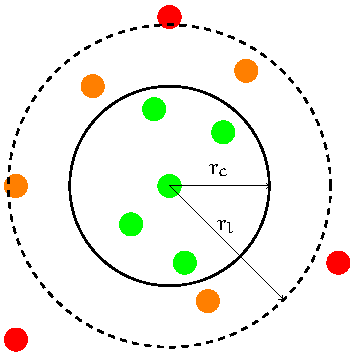
\includegraphics[width=0.42\textwidth]{./img/pairList/pairList}
	\caption{Schematic representation of the buffered pair--list construction respect to the central particle.
	Green particles are in the pair--list below the cutoff radius $r_c$, therefore included in the calculation of the interactions. Orange particles are in the pair--list for which at every step is checked if their distances became smaller then $r_c$. Red particles are not in the pair--list and they are completely neglected until the next list update.}
	\label{fig:pairlist}
\end{SCfigure}

A better performance can be achieved adding a dynamic update algorithm of the pair--list refresh rate during the simulation. A nice way is to consider the maximum distances traveled by a particles in the pair--list: if this distance is greater than $r_b = r_l - r_c$ then the pair--list is certainly updated. From this one can fix the refresh rate to a higher value increasing the performance.

\subsection{Thermostat algorithms} %Molecular Modelling, 382
A thermostat is an external tool that allows to maintain a system at a constant temperature.
%In \ac{MD} simulations if one want to use isothermal ensemble, so with constant temperature, some algorithms have to be developed in order to mimics the thermostat effect on the system and which generates the correct ensemble. 
Several algorithms are available. Some are based acting on particle velocities (Anderson, Berendsen, Bussi) other 
introduce some more \ac{DOF} in the system that take into account a real temperature bath coupling 
(Nosé--Hoover). We will describe in more detail the one used in this thesis work.

As suggested by Bussi \etal\, \cite{Bussi}, a common practice to implement a thermostat acting on particle 
velocities is related to a \textit{velocity rescale} algorithm in which the velocities of all particles are 
scaled by some factor. The simplest way is to consider the total kinetic energy $K$ of the system as in 
equation~\eqref{eq:kinetic} and the average kinetic energy $\ave{K}$ obtained from equation~\eqref{eq:kineticT} 
with the substitution $3N\rightarrow N_f$
\begin{equation*}
	\ave{K} = \frac{1}{2}N_f k_B T
\end{equation*}
where $N_f$ is the \textit{total} \ac{DOF} of the system and $T$ is the target temperature. Thus the scaling 
factor is defined by
\begin{equation*}
	\alpha_{T} \equiv \sqrt{\frac{\ave{K}}{K}}
\end{equation*}

The scaling operation is usually performed at a fixed rate during the simulation, or when the kinetic energy 
exceeds the limits of an interval centered around the target value. However the sampled ensemble is not 
explicitly known but, since in the thermodynamic limit the average properties do not depend on the ensemble 
chosen, even this very simple algorithm, often called \textit{weak coupling thermostat}, can be used to produce 
useful results. Despite this, for small systems or when the observables of interest are dependent on the 
fluctuations rather than on the averages or when other methods assume a canonical sampling, this method cannot be 
safely used.

In order to obtain the correct canonical sampling Bussi \etal\, \cite{Bussi} modify the way to calculate 
$\alpha_T$ so as to enforce a canonical distribution for the kinetic energy. The new scaling factor is obtained 
from
\begin{equation*}
	\alpha_{T} \equiv \sqrt{\frac{K_T}{K}}
\end{equation*}
where $K_T$ is extracted with a stochastic procedure from the equilibrium canonical distribution of the kinetic 
energy, given by
\begin{equation*}
	P(K_T)dK_T \propto K_T^{N_f/2-1}\ e^{-\beta K_T}\ dK_T
\end{equation*}
where $P(K_T)dK_T$ is probability that the system has a kinetic energy between $K_T$ and $K_T + dK_T$.

Since velocities are scaled only after some \ac{MD} steps this can cause a discontinuity in the particles 
velocities just before and after the scaling step. To avoid this problem, the authors suggest that the choice of 
$K_T$ can be based on the previous value of $K$ so as to obtain a smoother evolution. The procedure proposed by 
Bussi \etal\, consists in the following steps
\begin{itemize}
	\item Evolve the system for a single time step solving the equations of motion, so as to be in an $NVE$ ensemble;
	\item Calculate the total kinetic energy and evolve it for a single time step using an auxiliary continuous stochastic dynamics;
	\item Rescale the velocities by $\alpha_T$ so as to enforce this new value of the kinetic energy.
\end{itemize}

The authors have shown that an auxiliary dynamics for the kinetic energy of the form
\begin{equation*}
	dK = \frac{\ave{K} - K}{\tau_T}\ dt + 2 \sqrt{\frac{K\ave{K}}{N_f\tau_T}}\ dW
\end{equation*}
can do the job. Where $dW$ is a Wiener stochastic noise and $\tau_T$ is an arbitrary parameter which is related 
to the response time of the thermostat. In fact it reduces to the simple week coupling rescale if 
$\tau_T\rightarrow 0$ and to the Hamiltonian dynamics (as an $NVE$ ensemble) if $\tau_T\rightarrow +\infty$. 
Until the system is at non--equilibrium the first deterministic part is dominant an drives the system to 
equilibrium with a characteristic time $\tau_T$. Then the stochastic contribution samples the canonical 
distribution.
 

\subsection{Barostat algorithms} %Molecular Modelling, 382
As the thermostat maintains the system at a constant temperature $T$, a barostat is needed to maintain the system 
at a constant pressure $p$. To do this the system is coupled to a sort of piston so that changing the volume of 
the simulation box will adjust the pressure.

\subsubsection{Berendsen algorithm}
A common way, as proposed by Berendsen, is to scale both volume and particle coordinates. The rate of change of 
the pressure is given by
\begin{equation*}
	\frac{dp}{dt} = \frac{p_0 - p}{\tau_p}
\end{equation*}
where $p_0$ is the target pressure, $p$ is the instantaneous system pressure given by 
equation~\eqref{eq:pressure} and $\tau_p$ is a coupling constant related to the response time of the barostat. 
Thus if we consider a time step $\delta t$ then the volume scaling factor $\lambda$ is given by
\begin{equation*}
	\lambda = 1- k_T (p_0 - p) \frac{\delta t}{\tau_p}
\end{equation*}
where $k_t$ is the isothermal compressibility defined as
\begin{equation*}
	k_T = -\frac{1}{V}\left ( \frac{\partial V}{\partial p}\right )_{T}
\end{equation*}
while the factor $\nicefrac{\delta t}{\tau_p}$ gives a scaling factor for the isothermal compressibility that 
allow us to take into account the finite response time of the barostat. If $\tau_p \rightarrow 0$ the system has 
an infinity isothermal compressibility so it is necessary a really small change in volume to achieve the correct 
pressure; on the contrary if $\tau_p \rightarrow +\infty$ the system reduces to the Hamiltonian 
dynamics\footnote{If the system is coupled to a thermostat, then the canonical ensemble is sampled.}. The 
particle coordinates is scaled by the factor $\lambda^{\nicefrac{1}{3}}$.  

In the case of anisotropic system the pressure matrix $\mathbold{P}$ and the volume matrix $\mathbold{H}$ have to 
be considered and the Berendsen algorithm can be generalized such that even $\lambda$ becomes a $3\times 3$ 
matrix. However the main problem, as for the weak coupling thermostat, is that the sampled ensemble is not known. 
Thus a new approach, in order to correct sample the isobaric ensemble, has been derived by Parrinello and Rahman.

\subsubsection{Parrinello--Rahman algorithm}
The Parrinello--Rahman barostat \cite{ParrinelloBarostat1}\cite{ParrinelloBarostat2} is based on genuinely treat 
the coupling of the system to an external piston of ``mass'' $M_h$ through a Lagrangian method in which the 
volume becomes a Lagrangian variable of the system and its time evolution can be computed solving the 
Euler--Lagrange equations. Both the size and the shape of the simulation box are allowed to fluctuate. So it is 
perfectly compatible with anisotropic system. The shape and size of the simulation box are described by the 
volume matrix $ \mathbold{H}$ in equation~\eqref{eq:volumeMatrix} such that $V = |\det\mathbold{H}|$. 
$\mathbold{H}$ is the Lagrangian coordinate of the external piston. If the external pressure $p_0$ is applied to 
the piston then its potential energy is given by
\begin{equation*}
	U_p = p_0 |\det  \mathbold{H}|
\end{equation*}
instead, if $ \mathbold{H}$ varies in time then a ``kinetic energy'' is associated to the piston as follow
\begin{equation*}
	K_p = \frac{1}{2}M_h \text{Tr}(\leftidx{^t}{\dot{ \mathbold{H}}}{} \dot{ \mathbold{H}} )
\end{equation*}
where $\leftidx{^t}{(\cdot)}{}$ denote the transpose operation.

In order to write the Lagrangian of the system the particle coordinates must be expressed in terms of 
$\mathbold{H}$. This can be done defining the vector $\vec s_i$ so that $\vec r_i =  \mathbold{H} \vec s_i$. The 
square displacement can be obtained as $\vec r_i \cdot \vec r_i = \leftidx{^t}{ (\mathbold{H} \vec s_i)}{}  \mathbold{H} \vec s_i = \leftidx{^t}{\vec s_i}{} \leftidx{^t}{ \mathbold{H}}{}  \mathbold{H} \vec s_i$, often 
$\mathbold{G} = \leftidx{^t}{ \mathbold{H}}{} \mathbold{H}$. Parrinello \etal\, write the Lagrangian as follow
\begin{equation*}
	\mathcal{L} = \frac{1}{2}\sum_{i=1}^N m_i \dot{\vec s}_i \leftidx{^t}{\mathbold{G}}{} \dot{\vec s}_i - \sum_{i=1}^N \sum_{j=i+1}^N U_{ij}(\vec r) +  \frac{1}{2} M_h \text{Tr}(\leftidx{^t}{\mathbold{\dot H}}{} \mathbold{\dot H} ) -  p_0 |\det \mathbold{H}|
\end{equation*}
thus the equations of motion for $ \mathbold{H}$ and $\vec s_i$ can be computed solving the Euler--Lagrange 
equations. It can be shown that those equations of motion, derived in \cite{ParrinelloBarostat1} and 
\cite{ParrinelloBarostat2}, correct sample an isobaric ensemble. A practical way to show this is to consider the 
Hamiltonian of the system. Using equation~\eqref{eq:hamiltonian} the Hamiltonian is
\begin{equation*}
	\mathcal{H} = \frac{1}{2}\sum_{i=1}^N m_i \dot{\vec s}_i \leftidx{^t}{\mathbold{G}}{} \dot{\vec s}_i + \sum_{i=1}^N \sum_{j=i+1}^N U_{ij}(\vec r) +  \frac{1}{2} M_h \text{Tr}( \leftidx{^t}{\mathbold{\dot H}}{} \mathbold{\dot H} ) + p_0 |\det\mathbold{H}|
\end{equation*}
if the system is in equilibrium at temperature $T$, using the equipartition theorem, the kinetic term of the 
system particles contributes to the energy by $3Nk_BT/2$ while the kinetic term of the piston by $9k_BT/2$. Thus 
since $3N \gg 9$ the Hamiltonian can be approximated by
\begin{equation*}
	\mathcal{H} \simeq \ave{K} + U + p_0 V = H
\end{equation*}
that is the enthalpy. Since the Hamiltonian is a constant of motion the correct isobaric ensemble is sampled. If 
the system is also coupled to a thermostat, the $-TS$ term must be added, so the constant of motion become the 
Gibbs free energy $G = H - TS$ and the isobaric--isotherm ensemble is correctly sampled.

In order to understand the meaning of the $M_h$ parameter (the piston ``mass'') we report the dynamic equation of $\mathbold H$
\begin{equation*}
	M_h \mathbold{\ddot H} = V (p - p_0) (\leftidx{^t}{\mathbold{H}}{})^{-1}
\end{equation*}
The Parrinello--Rahman barostat is like a second order system. When there is an imbalance between the 
instantaneous internal pressure $p$ (see equation~\eqref{eq:pressure}) and the target pressure $p_0$, the system 
recovers this imbalance in a characteristic time governed by the parameter $M_h$. Since at equilibrium the 
properties of a system are independent of the masses of its constituent parts, $M_h$ can be arbitrarily chosen if 
one is interested only in static averages, otherwise a more appropriate choice must be made to obtain accurate 
dynamical properties. In this case, the authors suggest a choice of $M_h$ such that the relaxation time is of the 
order of $L/c$ where $L$ is simulation box size and $c$ is the sound velocity. 

Interesting is the fact that this algorithm can be generalized to an anisotropic pressure coupling making use of 
the theory of elasticity. Differently from the Berendsen algorithm, Parrinello--Rahman method is much slower in 
changing the volume until the equilibrium value is reached and it is less stable: if the system is not well 
equilibrated can lead to a large volume fluctuation with can compromise the simulation success. On the other hand 
the Parrinello--Rahman samples correctly the isobaric ensemble. A common strategy is to use the Berendsen 
barostat to reach equilibrium then switch to the Parrinello--Rahman algorithm to correctly sample the phase space 
associated to the isobaric ensemble.

\section{Empirical Force--Field model}
\label{sec:EmpiricalFF}
As we have seen in the previous section \ac{MD} provides a variety of tools for solving the time evolution of a 
$N$--particle system. Due to the possibility to capture different length and time scales \ac{MD} simulations can 
be used in a variety of systems, such as set of atoms, molecules or more complex system such as protein and 
macromolecules systems. In each of these systems, depending on the \textit{interaction model} and its 
\textit{parametrization}, we will be able to describe crucial molecular--level processes, such as hydrogen bond 
formation in organic molecules, which happen on the picoseconds time scale; or study slow processes such as the 
diffusion of massive colloidal particles, taking place on time scales of milliseconds if not seconds.

Considering soft or condensed mater, the most relevant for this thesis work, the main processes of interest 
ranging from protein folding to glass transitions, from surface diffusion to ligand--receptor binding take place 
on longer time scales (several ns) and involve a larger number of atoms ($N \gg 10^4$). In this case a crucial 
role is played by the \textit{Born--Oppenheimer approximation}. It says that we can separate the motion of the 
electrons by the motion of the atomic nuclei. This is done in order to integrate out the high frequency 
electrons' motions and to remove some \ac{DOF} due to the necessity to increase the time step and speed up the 
simulation. If, for some particular system, we want to know precisely the dynamics of the electrons we have to 
introduce quantum mechanical methods that are, even for a small number of particles ($N\sim 10^2$), very 
computationally time consuming. In the following, when we speak about atoms or chemical moieties we refer to it 
as for nuclei coordinates only without considering electrons at all.

Nevertheless atom or molecule interactions, such as bond formation, are mediated by the electron interactions. 
Thus, to describe the dynamics of such a system with a classical \ac{MD} tools and the Born--Oppenheimer 
approximation, it is necessary to develop an \textit{empirical model of the inter--atom interactions} that mimics 
the interactions behavior. Since forces are derived from the \ac{PEF}, a typical choice, when it is possible, for 
example with organic systems, is to model the inter--particle interactions by a set of pairwise addictive 
potentials that avoid any many--body calculations. Nevertheless for some systems this is impracticable, for 
example, for metal cores we need to consider the many--body calculations or an effective many--body potential 
that take into account the behavior of all metal atoms in the core. A typical solution is to use the many--body 
potential developed by Gupta (see \cite{Leach} for more details about metals treatment at \ac{MD} level). The set 
of functional forms of the inter--particle interaction potentials and its parameterization are collected into the 
so called empirical \acf{FF}. The meaning of \textit{empirical} is that most of the functional forms of the 
interactions has no ``first principle'' justification: they are chosen as a compromise between accuracy and 
computational efficiency. 
%Further it is necessary to stress out that a \ac{FF} is a well defined single entity containing the simulation parameters, the functional models of the interactions and also its parameterizations (and the way to obtain it). All the parameters of a \ac{FF} are in harmony to each other thus changing some parameters without retesting whole \ac{FF} is not allowed because, maybe, one can destroy the whole \ac{FF}.

For biomolecular applications two main classes of \acp{FF} exist: the \textit{atomistic} \acp{FF} in which basic 
particles are atoms, and the \textit{\ac{CG}} \acp{FF} in which the basic particles represent atom groups or 
small chemical moieties. In this case, even the way to realize the grouping, called \textit{mapping}, is part of 
the \ac{FF} itself. Different \ac{CG} \acp{FF} can use different mapping methods even with the same functional forms. 

In the following we will add some other information about \acp{FF} and describe the principal functional forms 
for modeling the inter--particle interactions and how to treat them in an \ac{MD} simulation. While in the next 
section we will focus on the main \ac{CG} \ac{FF} used in this thesis work: the \textacr{MARTINI} \ac{FF} 
developed by Marrink \etal\, \cite{Martini}.

\paragraph{\textbf{\textacr{parameterization}}} In general the functional forms for potential interactions are 
common to all particles in the system. The \ac{FF} is completed by a set of empirical parameters that 
characterize the interaction between different types of particles, whether they are atoms or whole chemical 
groups. Interaction parameters are empirical in the sense that they are assigned to reproduce a small set of 
target properties on a small group of systems. These target properties can be derived from experimental 
measurements or from finer--level calculations or simulations. Nowadays, atomistic and \ac{CG} biomolecular 
\acp{FF} come as ``packages'' of parameters and functional forms appropriate for the description of a large 
variety of chemical compounds in the liquid and solid phases.

\paragraph{\textbf{\textacr{transferability}}} As described above the parameterization of a \ac{FF} involves a 
small set of test systems for which some set of target proprieties are reproduced. The main characteristic of a 
\ac{FF} is the \textit{transferability} that means the ability of the model to describe different situations that 
differ from those used at the parameterization stage. Of course one would expect to be able to make some 
predictions for a bigger variety of systems and for other proprieties not used in the parametrization stage. 
Common faults of organic \acp{FF} concern, for example, phase transitions of organic compounds and phase 
transition temperatures.

\subsection{Inter--particles interactions}
For biomolecular applications the inter--particle interaction potentials are divided into two main classes: the 
\textit{bonded interactions} involving particles within the same molecules and the \textit{non--bonded 
interactions} engaging all particles in the system and which usually represent the Van der Waals and the 
electrostatic interactions. In the following the most common and general functional form for the \ac{PEF} is descried. In general the \ac{PEF} can be always splitted in a bonded and non--bonded contributions.
\begin{equation*}
	U(\vec r) = U_{\text{b}}(\vec r) + U_\text{nb}(\vec r)
	\label{eq:FFPEF}
\end{equation*}

The bonded contribution is generally described by the following terms
\begin{equation}
	\begin{aligned}
	U_{\text{b}}(\vec r) = &\frac{1}{2}\sum_{\text{bonds}} \frac{1}{2}k_i^b(l_i - l_{i0})^2\ + \frac{1}{2}\sum_{\text{angles}} k_i^a (\theta_i - \theta_{i0})^2 +\\
		 	& +\frac{1}{2}\sum_{\text{torsions}} V_n(1+\cos (n\omega - \gamma))
	\end{aligned}
	\label{eq:bondPEF}
\end{equation} 
the first two terms are harmonic potentials which model respectively the energy contribution due to the deviation 
from reference bond length $l_{i0}$ and a bond angle $\theta_{i0}$. $k_{bi}$ and $k_{ia}$ are the bond and angle 
elastic constants. The bond contribution involve a set of two particles in the some molecule while the angle 
contribution a set of three particles in the same molecule. The last term in equation~\eqref{eq:bondPEF} concerns 
the energy contribution due to the bond torsional change. It involves four particles in the same molecule and 
mimic the energy barrier needed to rotate the bond angle along the bond axis. $\omega$ is the torsional angle, 
$\gamma$ is a phase factor, $V_n$ qualitatively describes the energy barrier for each $n$--th components and $n$ 
is defined as the number of minima for each components.

The non--bonded contribution is described by the following terms
\begin{equation}
	U_\text{nb}(\vec r) = \sum_{i=1}^N \sum_{j>i} \left ( {4\epsilon_{ij} \left ( \left ( \frac{\sigma_{ij}}{r_{ij}} \right )^{12} - \left ( \frac{\sigma_{ij}}{r_{ij}} \right )^6 \right )  + \frac{q_iq_j}{4\pi\varepsilon_0 r_{ij}}} \right )
	\label{eq:nonbonPEF}
\end{equation}
The first term is the energy contribution due to the Van der Waals interactions modeled as a Lennard--Jones 
$12-6$ potential, fully characterized by the constants $\sigma_{ij}$ and $\epsilon_{ij}$ proper for each 
particles pair. The last term is the electrostatic energy contribution described by the particle charge $q$. The 
non--bonded interactions involve obviously all particles in the system, but for particles belonging to same 
molecule they are computed only if they are separated by at least three bonds, i.e. if their interactions are not 
described by bonded terms. The various contributions described above are schematically represented in 
figure~(\ref{fig:FFInteraction}).
\begin{figure}[!ht]
	\centering
	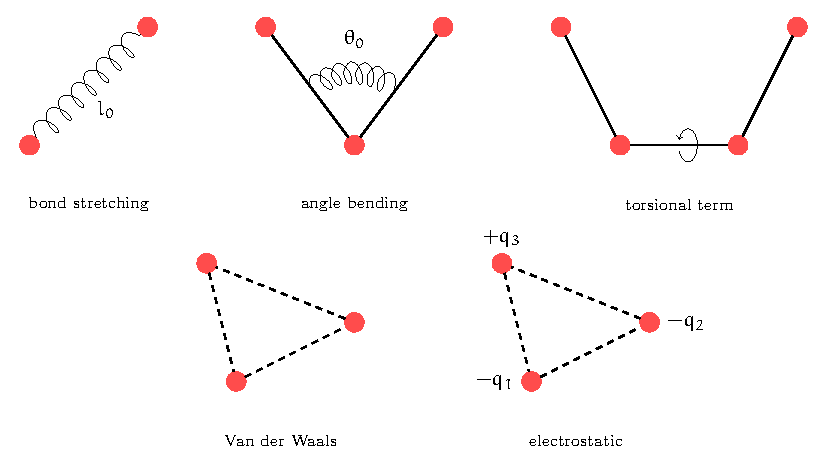
\includegraphics[width=0.8\textwidth]{./img/interPartInt/interPartInt}
	\caption{Schematic representation of the common inter--atom interactions for biomolecular applications: bond stretching, angle bending, torsional term, Van der Waals and electrostatic interactions.}
	\label{fig:FFInteraction}
\end{figure}

\subsection{Non--bonded interactions}
\label{sec:nonbonded}
The bonded interactions, as we can see in equation~\eqref{eq:bondPEF}, are at \textit{fixed range}, meaning that 
they depend, for example, on the equilibrium bond length that is fixed. Moreover, usually in standard \ac{MD} 
simulations the bond break is not taken into account. The same does not hold for the non--bonded interactions 
because they depend on the inter--particles distance $r_{ij}$ and they decay to zero as a power of $r_{ij}^{-d}$. 
Depending on the power order $d$ compared to the dimensionality $s$ of the system they are split into 
\textit{short range} if $d>s$ and \textit{long range} interactions if $1 \le d < s$. For example, as we shall see 
later, the Lennard--Jones $12-6$ potential decays to zero as $r^{-6}$ then it is a short range interaction, while 
the electrostatic is a long range interaction since it decays to zero as $r$.

\subsubsection{Cut--off, shift and switch methods}
As we have mentioned in section~\ref{sec:neighbor} the calculations of non--bonded interaction energy 
contributions is one of the most time consuming part of an \ac{MD} simulation. Even if we use a simple pairwise 
additive potential their calculation scale as $\sim N^2$. Thus, especially for short range interactions, various 
methods were developed in order to speed--up the simulation. The \textit{cut--off} method is the most used to 
treat the short range interactions and, in some cases, even the long range ones. Taking one particle into 
account, the general idea is to evaluate the non--bonded interactions with all other particles that are closer to 
the first for a distance $r_c$, called \textit{cut--off} radius, otherwise the interactions is set to $0$. This 
means that the new potential is of the form
\begin{equation*}
v^*(r) = \left \{
	\begin{aligned}
&v(r) & \quad & r \le r_c \\
&0    & \quad & r >   r_c
	\end{aligned} \right .
\end{equation*}

This generates a discontinuity in the potential and in its first derivatives, i.e. in the forces: this is bad for 
energy conservation. A trick for solving the discontinuity of the potential and to improve the energy 
conservation is to apply also a \textit{shift} of the potential value at $r_c$ so that $v^*(r_c) = 0$. Adding a 
constant will not affect the force calculations. The potential becomes
\begin{equation*}
v^*(r) = \left \{
	\begin{aligned}
&v(r) - v(r_c) & \quad & r \le r_c \\
&0    & \quad  & r >   r_c
	\end{aligned} \right .
\end{equation*}

Moreover, to solve the discontinuity of the forces, that can cause some instability, a simple possibility is to  
consider a linear term proportional to the first derivative of the potential, such as
\begin{equation*}
v^*(r) = \left \{
	\begin{aligned}
&v(r) - v(r_c) - \left . \frac{dv(r)}{dr}\right |_{r_c}\ (r - r_c) & \quad & r \le r_c \\
&0    & \quad  & r >   r_c
	\end{aligned} \right .
\end{equation*}
The shift methods can make the potential quite different from the original one. So this have to be properly taken 
into account in order to retrieve the correct thermodynamics proprieties.

Another powerful method to solve the discontinuity problem of the potential and forces is the \textit{switch} 
method. The general idea is to consider two cut--off radii  $r_{c1}$ and $r_{c2}$. If $r \le r_{c1}$ the original 
form is used; while if $r > r_{c2}$ the potential is set to zero. If $r_{c1} < r \le r_{c2}$ a \textit{switching 
function} is considered in order to \textit{smoothly} switch the potential to zero.

It is important to stress out that even the method used to treat the interactions, as the cut--off radii and 
eventually the switching function, are part of the simulation parameters that are, in turn, part of the \ac{FF}. 
So they are interdependent with the model parameterization, and should never be changed without retesting the 
target properties of the parameterization.

\subsection{Van der Waals interactions}
Van der Waals forces are a set of interactions that can be ascribed to quantum dynamic effects. In general they 
are described by a sum of a repulsive and an attracting term. The former effectually takes into account the Pauli 
exclusion principle between electron clouds; the latter is related to the dipole--dipole interactions (Keesom 
forces), dipole--induce dipole interactions (Debye forces), induced dipole--induced dipole interactions, London 
dispersion forces, hydrogen bonding and entropy effects, that involves both polar and non--polar atoms. 

The usual way to treat the Van der Waals interactions is to use a pairwise Lennard--Jones potential. The most 
common exponents for the attractive and repulsive contributions are $6$ and $12$, respectively. The former has 
physical meaning: calculating the repulsive part of the Van der Waals interaction for a simple system in a 
semi--classical approximation gives a potential energy contribution that vanishes as $r^{-6}$. While the latter 
is only for computational reason: giving the $r^{-6}$ term it is efficiency to calculate $r^{-12}$ as the square 
of $r^{-6}$. Thus it is just a common choice and other exponents can do the job, depending on the system in 
study. The general form for a $12-6$ Lennard--Jones potential is the following
\begin{equation}
	v(r) = 4\epsilon\left ( \left ( \frac{\sigma}{r}\right )^{12}  - \left ( \frac{\sigma}{r} \right )^6 \right ) = \frac{C_{12}}{r^{12}} - \frac{C_{6}}{r^{6}}
	\label{eq:lj126}
\end{equation}
where $C_{12} = 4\epsilon\sigma^{12}$, $C_{6} = 4\epsilon\sigma^{6}$ and $r$ is the pairwise particles distance. 
$\epsilon$ is related to the absolute value of minimum while $\sigma$ is related to the position of the minimum 
of the potential: $r_{\text{min}} = 2^{\nicefrac{1}{6}}\sigma$, often referred to by Van der Waals radius. These 
constants are proper for each particle pair. The attractive contribution is due to the negative part proportional 
to $r^{-6}$ while the repulsive one is due to the positive part proportional to $r^{-12}$. In 
figure~(\ref{fig:LG12511}) a plot of the function~\eqref{eq:lj126} with $\epsilon = \sigma = 1$ is shown.
\begin{figure}[!ht]
\centering
	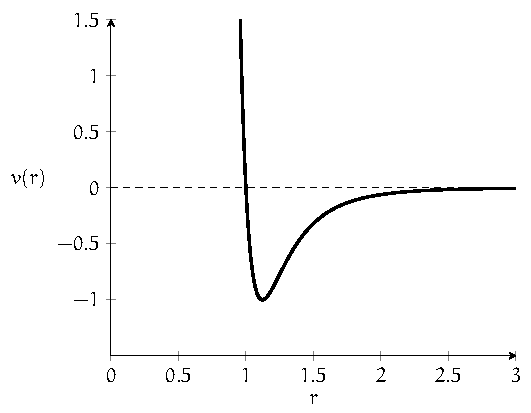
\includegraphics[width=0.6\textwidth]{./img/LJ126/LJ126}
	\caption{Plot of a Lennard--Jones interaction potential with $\epsilon = \sigma = 1$.}
	\label{fig:LG12511}
\end{figure}

The simplest and computationally most efficient way to treat a Lennard--Jones function, and in general all the 
short range interactions, is to use the cut--off method together with the shift or switch methods in order to 
obtain a continuous potential and/or a continuous forces. As we can see from figure~(\ref{fig:LG12511}) the 
Lennard--Jones potential vanishes rapidly with distance: at $r \sim 2\sigma$ its value is less then $1\%$ of the 
value in $r \sim \sigma$. A good choice for the cut--off is then of the order of $r_c \sim 2\sigma \div 3\sigma$.

\subsection{Electrostatic interactions}
\label{sec:longRangeInt}
Despite the long range characteristic of the electrostatic interaction, for computational efficient reason, most 
of the \acp{FF} for biomolecular applications treat them in the same way as a short range interaction by a 
cut--off method\footnote{In general, for computational reason, a common choice is to consider the same cut--off 
for Van der Waals and electrostatic interactions.}. Of course this is an approximation and can lead to serious 
issues in those proprieties or systems that strongly depend on the electrostatic interactions. As an example we 
report some situations in which the use of the short--range electrostatics can lead to artifacts: they are 
related to the development of a good polar solvent model (a good treatment of the electrostatic proprieties of 
water is really important for biological applications), as well as to the study of the interactions of charged 
particles with polar solvents, transport processes of charged moieties, calculations of the electrostatic 
potential inside macromolecules and so on. The calculation of the electrostatic energy contribution requires to 
take into account \textit{all particles} in a system, even all the periodic images due to the \ac{PBC}. This 
leads to a loss of computational efficiency.

If we consider only the simulation box the electrostatic energy contribution is
\begin{equation}
	U = \frac{1}{2}\sum_{i=1}^N\sum_{j\ne i}^N\frac{1}{4\pi\varepsilon_0}\frac{q_iq_j}{r_{ij}}
	\label{eq:electrostatic}
\end{equation}
where $q_i$ and $q_j$ are the charge of particles $i$ and $j$ and $r_{ij}$ is the distance between $i$ and $j$. 
But we need also all image boxes. Supposing, for simplicity, that the box is a cube of size $L$, then we can 
define a tern of integer numbers $(n_x,\ n_y,\ n_z)$, $n_i=0,1,2,\cdots$ so that the position of all other image 
boxes, with respect to the central simulation box, is $\vec n = L (n_x,\ n_y,\ n_z)$. Then the energy 
contribution becomes
\begin{equation}
	U = \frac{1}{2}\ \sideset{}{'}\sum_{n_x,n_y,n_z}^{+\infty}\ \sum_{i=1}^N\sum_{j=1}^N\frac{1}{4\pi\varepsilon_0}\frac{q_iq_j}{\|\vec r_i - \vec r_j + \vec n \|}
	\label{eq:electrostaticImage}
\end{equation}
where the prime indicates that for $\vec n = 0$, i.e. the energy contribution of the simulation box, we need to 
exclude the self interaction term: in the inner sum it must be $j \ne i$.

As described above, a cut--off method is a good easy way to solve equation~\eqref{eq:electrostatic} and sometimes 
it produces sufficiently good results. However, the increasing of computer power can lead to develop more 
rigorous methods to solve equation~\eqref{eq:electrostaticImage}, even for very large systems. The main problem 
is that the summation in equation~\eqref{eq:electrostaticImage} is \textit{conditionally convergent}\footnote{A 
conditionally convergent series contains both positive and negative terms such that the positive or negative term 
alone form both a divergent series. The sum of a conditionally convergent series depends on the order in which 
the positive and negative terms are considered.} and converges extremely slowly so that it would need so many 
terms to converge that its computational cost would be too high, especially for large systems (of the order of 
$N > 10^4$). The most important methods developed to solve this problem are based on the \ac{ESM}. We shall 
describe those used in this thesis work: the \ac{ESM} itself and the \ac{PME} method. For a more complete 
discussion about the advanced methods developed to treat the electrostatic interactions for biological 
applications the reader is addressed to the review by Cisneros \etal\, \cite{Cisneros}.

\subsubsection{Ewald summation method} %Molecular Modelling, 334
The \acf{ESM} is the first method introduced by Ewald for a correct treatment of the electrostatic energy 
contribution in an ionic crystal. The basic idea is to split the summation in equation~ 
\eqref{eq:electrostaticImage} in two series both rapidly convergent. The method is based on the following identity
\begin{equation}
	\frac{1}{r} = \frac{f(r)}{r} + \frac{1 - f(r)}{r}
	\label{eq:ewaldTrick}
\end{equation}
the trick is to choose a function $f(r)$ that will deal with the rapid variation of the $1/r$ term for small $r$ 
and the slow decay at long $r$; in that case the two series can rapidly converge.
\begin{figure}[!ht]
	\centering
	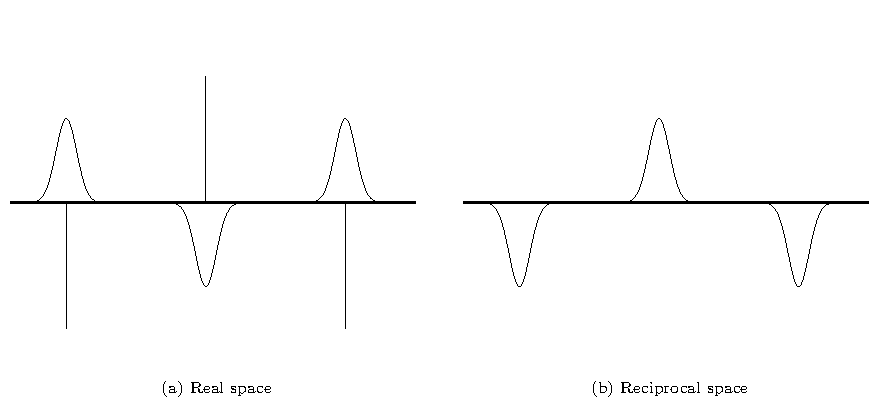
\includegraphics[width=0.8\textwidth]{./img/EwaldSum/EwaldSum}
	\caption{Schematic illustration of the \acs{ESM} charge distribution: in (a) point charges (represented by vertical lines) and the neutralizing Gaussian charge distribution; in (b) the counteracting Gaussian distribution.}
	\label{fig:ewald}
\end{figure}

The \ac{ESM} for electrostatic interactions works, as illustrated in figure~(\ref{fig:ewald}), considering each 
point--like charge in the system surrounded by a neutralizing charge distribution of equal magnitude but opposite 
sign that decays rapidly to zero. Simplifying the notation for a one dimensional system, the simplest functional 
form is a Gaussian distribution centered in the position $r_i$ of the point--like charge $q_i$, of the form
\begin{equation}
	\rho_i(r) = \frac{q_i\alpha^3}{\pi^{3/2}}e^{-\alpha^2 (r - r_i)^2}
\end{equation}
that obeys the relation
\begin{equation*}
	\frac{q_i\alpha^3}{\pi^{3/2}}\int_{r_i-\epsilon}^{r_i+\epsilon}e^{-\alpha^2 (r - r_i)^2}\ dr \simeq q_i
\end{equation*}
where $(r_i-\epsilon; r_i+\epsilon)$ is a small interval around $r_i$. The energy contribution due to this set 
up, the point--like charge \textit{and} the gaussian charge distribution, is given by
\begin{equation}
	U_r = \frac{1}{2}\sum_{i=1}^N\sum_{j=1}^N\ \sideset{}{'}\sum_{n_x,n_y,n_z}\ \frac{q_iq_j}{4 \pi \varepsilon_0} \frac{\erfc{(\alpha \| \vec r_i - \vec r_j + \vec n \|)}}{\| \vec r_i - \vec r_j + \vec n \|}
	\label{eq:ewaldReal}
\end{equation}
where the prime indicate that for $\vec n = 0$ must be $i\ne j$, $\erfc{(x)} = 1-\erf{(x)}$ is the complementary 
error function and $\erf{(x)}$ is the error function. They are given by
\begin{equation}
	\erfc{(x)} = \frac{2}{\sqrt{\pi}}\int_{x}^{+\infty} e^{-t^2}\ dt, \qquad \erf{(x)} = \frac{2}{\sqrt{\pi}}\int_{0}^{x} e^{-t^2}\ dt
	\label{eq:erf}
\end{equation}

The point is that the summation involving the complementary error function in equation~\eqref{eq:ewaldReal} is 
rapidly convergent and it needs very few terms so that a cut--off method can be safely used. The rate of 
convergence depends on the $\alpha$ parameter: the bigger is $\alpha$, the more rapidly the series converges and 
the shorter the cut--off radius can be. Thus the \ac{ESM} use the $\erfc{(r)}$ as $f(r)$ function in 
equation~\eqref{eq:ewaldTrick}. Of course since we added a non physical neutralizing charge in the system, in 
order to restore the real charge distribution, we must consider another distribution, called counteracting charge 
distribution, of equal magnitude but opposite sign. Considering the identity in equation~\eqref{eq:ewaldTrick} 
this lead to an energy contribution $U_f$ of the form $(1-f(r))/r$. But using equation~\eqref{eq:erf}, it becomes 
of the form $\erf{(r)}/r$. Another important trick is to compute $U_r$ in the \textit{real space} while $U_f$ in 
the \textit{reciprocal space}, thus considering its Fourier transform. This energy contribution is given by
\begin{equation}
	U_f = \frac{1}{2}\sum_{i=1}^N\sum_{j=1}^N\ \sum_{k_x,k_y,k_z}\ \frac{1}{4\pi\varepsilon_0}\frac{4\pi}{L^3k^2}e^{-k^2/(4\alpha^2)}e^{\mathsf{i}{\vec k \cdot (\vec r_i - \vec r_j)}}
	\label{eq:ewaldReciprocal}
\end{equation}
where $\vec k = 2\pi\vec n/L$ are the reciprocal lattice vectors. Even $U_f$ converges rapidly as $U_r$ in 
equation~\eqref{eq:ewaldReal}; then a cut--off method can be safely used. Nevertheless, opposite to $U_r$, the 
smaller is $\alpha$, the shorter the cut--off can be. Clearly a proper \textit{balance} between the real and 
reciprocal space summation is needed.

Since in equation~\eqref{eq:ewaldReal} even the self interaction with each Gaussian is included we need to add 
another item for cancel it out; this is done by the self--term
\begin{equation}
	U_\text{self} = -\frac{\alpha}{\sqrt{\pi}}\sum_{i=1}^N\frac{q_i}{4\pi\varepsilon_0}
	\label{eq:EwaldselfTerm}
\end{equation}

Summarizing, the energy contribution of the electrostatic interactions by the \ac{ESM} is computed summing 
equations~\eqref{eq:ewaldReal},\eqref{eq:ewaldReciprocal} and~\eqref{eq:EwaldselfTerm} to obtain
\begin{equation}
	\begin{aligned}
		U =&\quad\frac{1}{2}\sum_{i=1}^N\sum_{j=1}^N\ \sideset{}{'}\sum_{n_x,n_y,n_z}\ \frac{q_iq_j}{4 \pi \varepsilon_0} \frac{\erfc{(\alpha \| \vec r_i - \vec r_j + \vec n \|)}}{\| \vec r_i - \vec r_j + \vec n \|}\ + \\
		 &+ \frac{1}{2}\sum_{i=1}^N\sum_{j=1}^N\ \sum_{k_x,k_y,k_z}\  \frac{1}{4\pi\varepsilon_0}\frac{4\pi}{L^3k^2}e^{-k^2/(4\alpha^2)}e^{\mathsf{i}{\vec k \cdot (\vec r_i - \vec r_j)}}\ + \\
		 &- \frac{\alpha}{\sqrt{\pi}}\sum_{i=1}^N\frac{q_i}{4\pi\varepsilon_0}
	\end{aligned}
	\label{eq:EwaldEnergy}
\end{equation}
The first line is the real space contribution while the second is the Fourier energy contribution. Since the last 
self--interaction term is constant it does not affect forces computation. The \ac{ESM} offers a well defined 
method to properly treat electrostatic interactions, nevertheless it is quite expensive in term of computational 
resources. If $\alpha$ and the cut--off are constant, then the computation scales as $\sim N^2$.

For biomolecular applications most \ac{MD} tools set an equal cut-off radius for both Van der Waals interaction and the real part of the Ewald summation~\eqref{eq:EwaldEnergy} in order to achieve for both a scaling of the order $\sim N$. However in this way the computation of the reciprocal part in the Ewald summation~\eqref{eq:EwaldEnergy} will be very inefficient as it scales as $\sim N^2$. In order to increase the efficiency of the calculation of the Fourier transform various of advanced methods can be used. They are all based on the use of the \ac{FFT} method. In this way the reciprocal part can scale as $\sim N\ln N$. Since \ac{FFT} requires discretized quantities, the idea of such methods, called \textit{particle mesh} is to consider the charge density spread on a mesh grid and then evaluate the electrostatic potential via solving the Poisson's equation\footnote{Given a charge distribution $\rho(\vec r)$ then the associated electrostatic potential $\phi(\vec r)$ can be calculated solving the Poisson's equation $\displaystyle \nabla^2\phi(\vec r) = -\frac{1}{\varepsilon_0} \rho(\vec r)$. If a charge $q$ is at position $\vec r$ its electrostatic potential energy is given by $U = q\phi(\vec r)$.} using fast Poisson solver together with the \ac{FFT} method; this can be done, for example, exploiting the \ac{PBC} in order to discretize and make periodic the Poisson's equation.
%\footnote{It is generally true that the Poisson's equation become ``easily'' solvable in Fourier space. Considering a one dimensional Poisson's equation, its Fourier transform is $k^2\varepsilon_0\tilde\phi(k) = \tilde \rho(k)$ where $\tilde\phi(k)$ and $\tilde\rho(k)$ are, respectively, the Fourier transform of the electrostatic potential and charge distribution.}.
Such algorithms include the \textit{particle--particle particle--mesh} method, \textit{particle mesh Ewald} 
method, \textit{fast--Fourier Poisson} method and a recent methodology based on multi--scale mesh grid. The 
efficiency and accuracy of such mesh--based algorithms depends strongly on the way in which the charges are 
attributed to the mesh points, this makes the methods different. In the following we will describe the one used 
in this thesis work, the \acf{PME} method.

\subsubsection{Particle mesh Ewald method}
\acf{PME} method developed by Darden \etal\, \cite{DardenPME} is based on the \ac{ESM} so the starting point is 
equation~\eqref{eq:EwaldEnergy}. As described above, the first part of the Ewald summation is computed in the 
real space together with the Van der Waals contribution using the same cut--off radius. The reciprocal part 
instead, is computed using \ac{FFT} method, in order to have a gain of performance. First, we need to 
consider a grid mesh onto which the Gaussian counteracting charge distribution is spread. The basic idea, then, 
is to calculate the electrostatic energy solving Poisson's equation through \ac{FFT} methods. The efficiency and 
accuracy depend on the way the charges are distributed onto the grid. To do this a \textit{charge assignment 
function}, $W(r)$ is introduced such that, considering for simplicity a one dimensional system, the fraction of a 
charge at position $r$ assigned to a grid point at position $r_p$ is given by $W(r_p - r)$. Hence, if we have a 
charge density $\rho(r)$ then the charges at the grid point $r_p$ are given by
\begin{equation}
	q_M(r_p) = \int_0^L\ W(r_p - r) \rho (r)\ dr
	\label{eq:meshAssign}
\end{equation}
where $L$ is the box length and, if $h$ is the grid spacing, $M = L/h$ is the number of mesh point. In 
figure~(\ref{fig:gidAssign}) the charges assignment is schematically represented. 

The assignment function should have the following proprieties: it should be an even function and it should be 
normalized in such a way that the sum of the fractional charges equals the total charge of the system. Moreover 
the best accuracy is obtained with a dense grid in order to reduce as much as possible the discretization of the 
charge density. However the computational cost increases as the number of grid points: a balance between 
efficiency and accuracy is clearly needed.
\begin{SCfigure}
	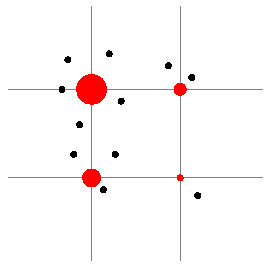
\includegraphics[width=0.35\textwidth]{./img/gridCharge/gridCharge}
	\caption{A schematic representation of the charge assignment. The black filled circles are a unit particle charge, while the red ones, are the charges assigned to grid points. The bigger is the circle, the more is the charge.}
	\label{fig:gidAssign}
\end{SCfigure}

A nice way to solve the problem of charge assignment is to shift the problem to the discretization of the Fourier 
transform. This can be viewed as an interpolation problem. Consider the $e^{-\mathsf{i}\vec k\cdot \vec r_j}$ 
term in the Fourier transform of equation~\eqref{eq:ewaldReciprocal}. In general $\vec r_j$ does not correspond 
to a mesh grid point, so that term is not part of a discrete Fourier transform. The idea, thus, is to interpolate 
it in terms of values of the complex exponential at the mesh points. Switching for simplicity to a one 
dimensional system, if the mesh grid has $M = L/h$ points, a particle coordinate $r_j$ is located between mesh 
points $[r_j/h]$ and $[r_j/h] + 1$ where $[\cdot]$ denotes the integer part; thus a $p$--order interpolation of 
the exponential is of the form
\begin{equation*}
	e^{-\mathsf{i}kr_j} \simeq \sum_{i=1}^M W_{p}\left ( \frac{r_j}{h} - i \right ) e^{-\mathsf{i}khi}
\end{equation*}
where $W_{p}$ denotes the interpolation coefficient. A $p$--order interpolation means that only the $p$ mesh 
points nearest to $r_j$ contribute to the sum. Assuming a point--like charge distribution the Fourier transform 
of the charge density is therefore
\begin{equation*}
	\rho_k \simeq \sum_{i}e^{-\mathsf{i}khi} \sum_j\ q_iW_{p} \left ( \frac{r_j}{h} - i \right )
\end{equation*}
we can interpret the above expression as the discrete Fourier transform of the charge density
\begin{equation*}
	\rho(i) = \sum_j\ q_iW_{p} \left ( \frac{r_j}{h} - i \right )
\end{equation*}
but using equation~\eqref{eq:meshAssign}, it is nothing that the point--like charge distribution assigned to the 
mesh point $i$ through the assignment function $W_{p}$.

We clearly see that the charge assignment problem is now shifted to the complex exponential interpolation. There 
are two main methods to make the interpolation: the \textit{Lagrange interpolation method} and the \textit{Euler 
SPLINE interpolation method}. The basic idea of the former is to use, as interpolating function, a polynomial 
function of degree $ \le (n-1)$ where $n$ is the number of points to interpolate, that passes through all the $n$ 
points, and which is constructed with a summation over the \textit{Lagrange basis polynomials} as follow
\begin{equation*}
	P(x) = \sum_{i=1}^n y_i \prod_{\substack{k=1\\k\ne i}}^n \frac{x-x_k}{x_i - x_k}
\end{equation*}
where $(x_i;y_i)$ are the sets of points to interpolate. The main disadvantage of this method is that, even if 
$P(x)$ is continuous everywhere, its derivative is not, thus it can lead to some instability in \ac{MD} 
simulations.

The latter method, that is the most used in \ac{MD} tools, is based on the concept of \textit{SPLINE 
interpolation}. Instead of using a unique interpolating function that passes through each point, the SPLINE 
method uses a \textit{piecewise polynomial function}, called SPLINE, in which each piece is smoothly connected 
and optimized to interpolate a subset of the points. The Euler SPLINE method use the \textit{exponential Euler 
SPLINE} that is constructed with the basis of the Euler $n$--degree polynomials $A_n(x;\lambda)$ generated by the 
following equation
\begin{equation*}
	\frac{\lambda - 1}{\lambda - e^z}e^{xz} = \sum_{n=0}^{+\infty} \frac{A_n(x;\lambda)}{n!}z^n
\end{equation*}
where $\lambda$ is a complex parameter and $z$ is a complex variable. The main properties of such SPLINE is that, 
it is $n-1$ times analytic, continuously differentiable and then can solve the instability problem of the 
Lagrange interpolation method. In literature the Euler SPLINE method is referred to as \textit{smooth} \ac{PME} 
and the reader is addressed to the article by Essmann \etal\, \cite{EssmannSPME} for more technical details about 
the interpolation procedure.

Summarizing, the \ac{PME} method is implemented with the following scheme
\begin{itemize}
	\item By the interpolation of the complex exponential in the Fourier transform of the Ewald summation, the 
		  Gaussian counteracting charge distribution are spread onto the mesh grid;
	\item Poisson's equation for the discretized charges are solved through the \ac{FFT} methods;
	\item The $U_f$ energy contribution is obtained considering the inverse Fourier transform;
	\item Electrostatic forces are computed and assigned to the charged system particles.
\end{itemize}

The main advantages of the \ac{PME} algorithm are that the potential energy and forces are smooth functions of 
the particles positions. The method offers a good energy conservation and offers a good balance between accuracy 
and computational efficiency since it scales as $\sim N\ln N$. Moreover, despite we have described \ac{ESM} and 
\ac{PME} applied to the electrostatic interaction, they can be used, with some changes, with all long--range 
interactions and in general to all energy contributions that decay as $r^{-d}$, for example, even with the Van 
der Waals energy contribution.

\subsection{Charge representation}
\label{sec:chargeRep}
Even if some methods, such as the \ac{PME} one, have been developed to speed up the computation of electrostatic 
energy contribution one of the main problems of \acp{FF} for biomolecular applications remains the \textit{charge 
representation}: the way in which the charges of atoms or molecules are assigned to the system particles. The 
problem arises from the necessity to represent the electron clouds and the interactions that generate. 
Nevertheless this is crucial for a better description of most electrostatic phenomena such as polarizability of 
molecules and polar solvent, solvation shell of charged ions, protein--ligand interactions, ion transport through 
polar and non--polar medium, self assembly processes and so on.

The most common solution is the \textit{atom--centered ``partial charge'' approximation} in which the full charge 
density of the molecule is replaced by fractional point--like charges assigned to each atom of the molecule. 
Traditionally most non--polarizable \acp{FF} (as those we will use in this thesis work) assign to each atom of a 
molecule a fixed partial--charge. The most used procedure for extracting partial--charges from molecular wave 
functions is based on fitting atomic charges with the molecular electrostatic potential, computed with \textit{ab 
initio} calculation such as \textit{density functional theory}. The fitting procedure consists in minimizing the 
deviation between the electrostatic potential produced by the assigned charge and the molecular electrostatic 
potential. Such representation is believed to be an important source of error in the electrostatics treatment. 
Moreover with fixed charge assignment it is impossible to take into account those phenomena that involve a 
transfer of charge inside the molecule, as polarization effect. The use of off--centered charges and/or higher 
order atomic multipoles can significantly improve the treatment of electrostatics but of course it is necessary a 
good balance between accuracy and performances since the electrostatic problem can rapidly drive to a loss of 
computational efficiency.

\subsection{Polarization}
\label{sec:polarization}
Polarization refers to the redistribution of the electron charge density of a molecule in presence of an external 
electric field, generated, for example, by charged ions or by another molecule. Polarization is responsible to 
non--additive attractive inter-- or intra--molecular interactions which have many--body characteristics. These 
effects have been recognized to have an important role in many biological interactions in which different 
compounds are present. An increasing number of studies show that the lack of these effects can lead to serious 
limitations, particularly, for systems that involve different environments such us water and proteins or water 
and lipids. In \ac{MD} simulations polarization effects are included using either \textit{implicit} or 
\textit{explicit} methods.

The implicit method completely avoids the many--body calculations by including a mean polarization effect in the 
functional form of the interaction potential. The general idea is to surround all the simulation box by a 
transparent medium with a relative dielectric constant $\varepsilon_r$. In this way the polarization effect is 
taken into account considering a mean field theory and solving the Poisson's equation to determine the 
electrostatic potential due to system charges by the substitution 
$\varepsilon_0\rightarrow\varepsilon_0\varepsilon_r$. Since it avoids many--body calculations, this method gives 
an incomparable gain in performances but it must be carefully used. The main disadvantage is that the mean 
polarization effect is added to all system particles and this wash out all the details about a possible 
polarization effect in a molecule. Moreover the electrostatic interaction between charged particles is affected 
by the mean field effect. This produce a correct electrostatic interaction for particles inside the same solvent 
for which the implicit medium is parameterized. Otherwise, if the simulation box is composed by different 
chemical environments such as a polar and non--polar compounds, using the same dielectric constant would lead to 
badly calculate the electrostatic interactions for particles in the non--polar environment. Thus, this method can 
be safely used when our system is composed principally by one kind of solvent, for example water. 

The way to correct the above behavior is to use an explicit method. As the name suggests, the polarization effect 
is taken into account for every molecule in the system by an its proper model included in the \ac{FF}. The 
general idea is to add some more internal \ac{DOF} to a molecule or atom to take into account the movement of 
charges and/or split the point--like charge assigned, for example, to a chemical group, to a partial-charge 
assigned to each particles of the chemical group itself. This can be done for every molecule or atom in the 
system and thus it is the optimum to better describe systems with different chemical environments. Obviously this 
method is more time consuming compared to the first. 

%\subsection{Atomistic model}
\subsection{Coarse--Grained model}
\label{sec:CGModel}
As we have introduced at the beginning of this section, for biomolecular applications two main classes of \acp{FF} exist: atomistic \acp{FF} and \ac{CG} \acp{FF}. Since the atomistic model takes into account all the atoms in a molecule it is obviously the most real and accurate \ac{FF}. Nevertheless the number of \ac{DOF} of the system increases leading to a loss of performances. Moreover, basically, the atomistic \acp{FF} are efficient until the physical proprieties can be properly sampled on a time scale of a few microseconds over a length scale of a few nanometers. As the time and length scales increase more and more time is needed to carry out a complete simulation. Unfortunately many biological processes involving lipid membranes and other organic molecules, including synthetic compounds, take place on much longer time and length scales.

One possible solution is to \textit{integrate out} some \ac{DOF}, preserving those that are relevant for the problem in exam: this procedure is called \textit{coarse--graining}. The basic units of \ac{CG} \acp{FF} are called \textit{beads}, each representing a group of atoms or a well defined chemical moiety. The size of the group of atoms that is represented by a single bead determines the degree of coarsening of the \ac{FF}. Even in this case, all the general features described above, apply: functional forms need to be chosen and their parameterization need to be adjusted so as to reproduce the desired target properties. Moreover, in this case, even a \textit{mapping} procedure should be defined as the first step in the development of a \ac{CG} model: This establishes a link between the atomistic model and the coarse--grain beads. There is not a unique or correct procedure to obtain the mapping because it depends on the desired coarse--graining level, on the time and length scales that one wants to correctly sample and on the properties one wants to reproduce. For biological applications \ac{CG} \acp{FF} are often designed to reproduce specific thermodynamics properties such as surface tension, free energy of partitioning, free energy of hydration and so on, instead of, for example, the structural properties.

In general a \ac{CG} \ac{FF} is more computationally efficient than an atomistic one for the following reasons: the \ac{DOF} of the system are reduced due to the \ac{CG} procedure and a smaller number of interactions and forces has to be taken into account; bead--bead interactions, which result from the removal of finer structural details, are softer than atom--atom interactions. Thus, vibrational modes are slower, and their sampling can be achieved using larger \ac{MD} time steps than in atomistic simulations; softer interactions imply a smoother \ac{PEF} which leads to faster diffusion.

\section{MARTINI: a Coarse--Grained Force--Field}
\martini is a \ac{CG} \ac{FF} originally developed by Marrink \etal\, \cite{Martini} for organic solvents and lipids and then extended to proteins \cite{MartiniProtein}, carbohydrates \cite{MartiniCarbo} and a broad class of polymers \cite{MartiniPolymers}. The original aim was to improve the description of the physical and chemical properties of lipid membranes using a \ac{CG} model. The power of the model was immediately clear and soon its philosophy was changed to develop a \ac{FF} applicable to a broad range of organic system providing a set of extensively calibrated building blocks to construct a large variety of organic molecules without reparametrizing the \ac{FF}. This is possible, because, instead of focusing on accurately reproducing structural details of a particular system, the \ac{FF} is based on accurately reproducing the interaction between polar and non--polar chemical compounds. This is the main target property: The \textit{partitioning free energy} between water and a large number of organic solvents, i.e. the free energy of transfer of chemical moieties from polar and non--polar solvents. These building blocks are representative of the main chemical moieties in an organic system, this is the guide for the mapping procedure.

\subsection{Mapping}
The mapping of the \martini beads, is based on a four--to--one scheme that groups four heavy atoms like C, S, O and so on, plus their associated hydrogen atoms, into a single interaction site. Consistently four water molecules are modeled with one \martini bead. An example of the coarse-graining procedure including both atomistic and \ac{CG} descriptions is shown in figure~(\ref{fig:martiniMapping}).
\begin{figure}[!ht]
	\centering
	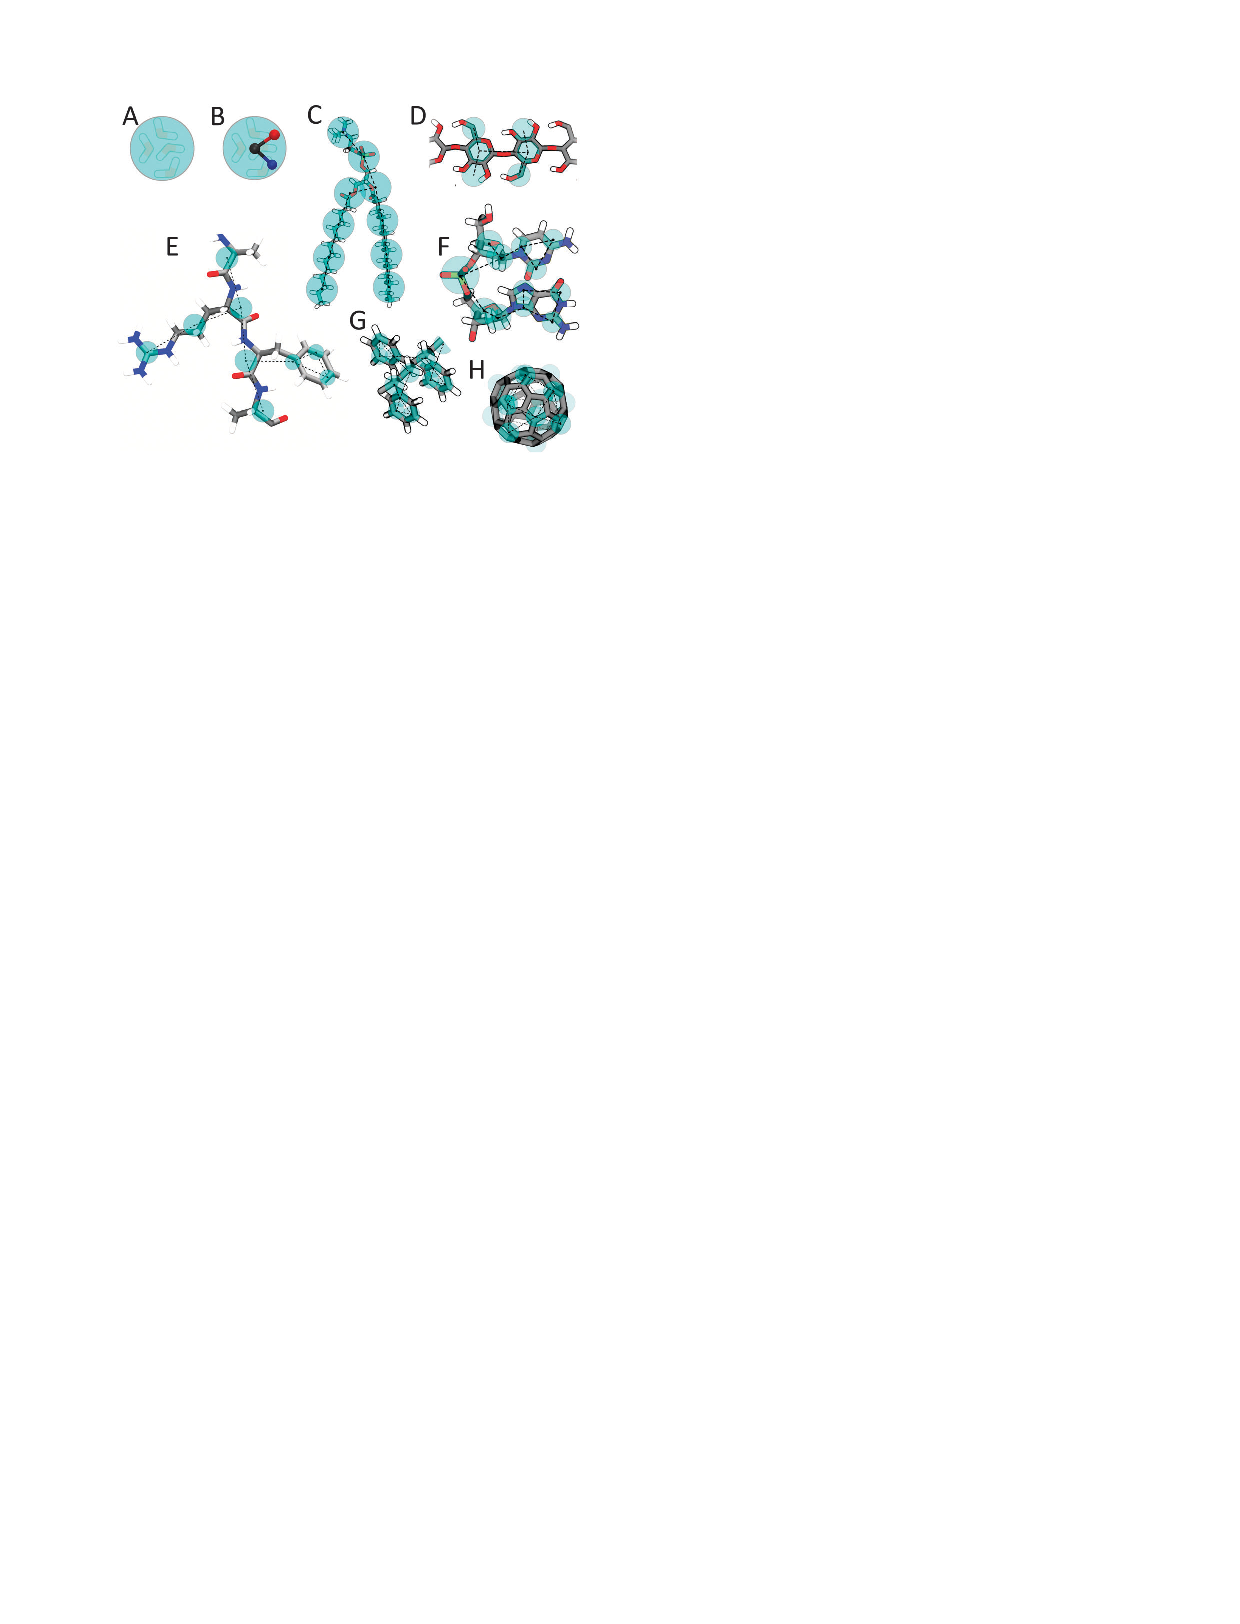
\includegraphics[width=0.5\textwidth]{img/martiniMapping}
	\caption{\martini mapping and atomistic structures compares of some molecules: (A) Standard water bead, (B) polarizable water bead, (C) \acs{DMPC} lipid, (D) Polysaccharide fragment, (E) Peptide, (F) \acs{DNA} fragment, (G) Polystyrene fragment and (H) Fullerene molecule. In all cases \martini \acs{CG} beads are shown as cyan transparent beads overlaying the atomistic structure. Taken from \cite{MartiniReview}.}
	\label{fig:martiniMapping}
\end{figure}

There are four main bead types: polar (P), non--polar (N), apolar (A) and charged (Q). Each bead type has a number of subtypes to take into account a more accurate representation of the chemical nature of the moieties due to underlying the specific atomistic structure. These subtypes are distinguished by the hydrogen bonding capabilities: donor (d), acceptor (a), both donor and acceptor (da) and none ($0$) and/or by their degree of polarity: lowest polarity ($1$), $\cdots$, highest polarity ($5$).

\begin{SCtable}\footnotesize
	\begin{tabular}{lc}
		\toprule
		Level  & $\epsilon$\,[kJ/mol] \\ \midrule
		O	   & $5.6$	 \\ \midrule
		I      & $5.0$	 \\ \midrule
		II	   & $4.5$	 \\ \midrule
		III	   & $4.0$	 \\ \midrule
		IV	   & $3.5$	 \\ \midrule
		V	   & $3.1$	 \\ \midrule
		VI	   & $2.7$	 \\ \midrule
		VII	   & $2.3$	 \\ \midrule
		VIII   & $2.0$	 \\ \midrule
		IX     & $2.0$	 \\ \bottomrule
	\end{tabular}
	\caption{Interaction strength parameter ($\epsilon$). The last one is for the special case $\sigma=0.62$~nm.}
	\label{tab:martiniEpsilon}
\end{SCtable}

\subsection{Interactions potential}
\paragraph{\textbf{van der waals interactions}} The functional form describing pairwise Van der Waals interaction is a Lennard--Jones $12-6$ potential as in equation~\eqref{eq:lj126}.
%The $\epsilon$ and $\sigma$ parameters are first obtained for a same--type interactions and then the inter--type parameters are computed as follow
%\begin{equation*}
%	\epsilon_{ij} = \sqrt{\esilon_{ii}\epsilon_{jj}} \qquad \sigma_{ij} = \frac{1}{2}(\sigma_{ii} + \sigma_{jj})
%\end{equation*}
For most beads the $\sigma$ parameter is set equal to $0.47~$nm except for the Q--C$_1$ and Q--C$_2$ interactions for which $\sigma = 0.62$~nm. This is consistent with reproducing the hydration shell when a charged bead (Q) is dragged into an apolar medium. The strength of the interactions is instead dived into ten levels, reported in table~(\ref{tab:martiniEpsilon}). The association of the interactions strength with the \martini beads is shown in figure~(\ref{fig:martiniInteractions}).
\begin{figure}[h!t]%
	\center
	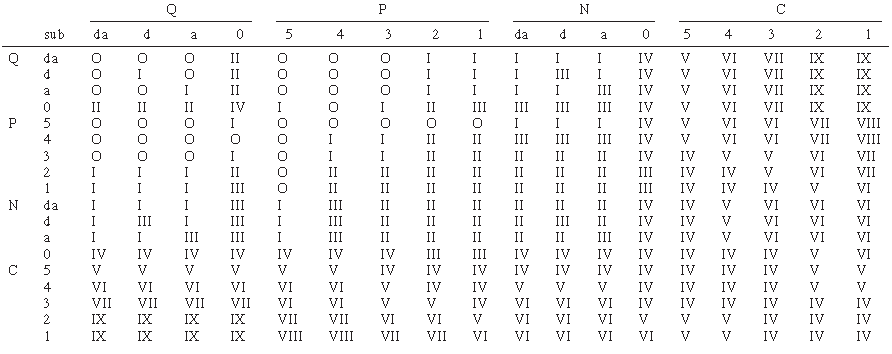
\includegraphics[width=\textwidth]{img/martiniInteractions.pdf}%
	\caption{Interaction strength association matrix for the \martini bead types and subtypes. Taken from \cite{Martini}.}
	\label{fig:martiniInteractions}
\end{figure}

% \begin{adjustwidth}{-3cm}{-5cm}%
% \centering
% \begin{minipage}[c]{1.2\textwidth}%
% 	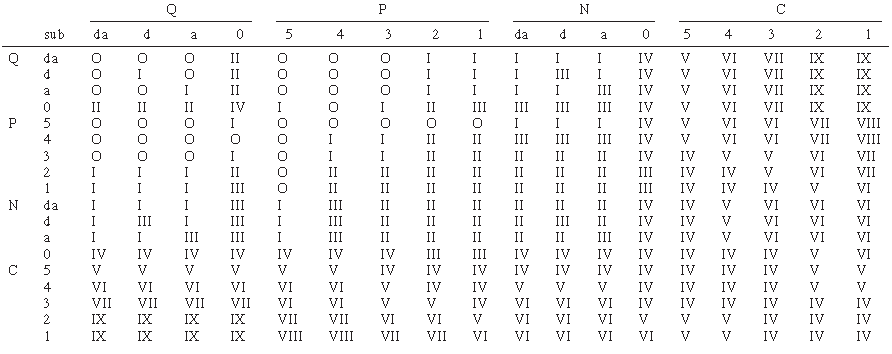
\includegraphics[width=\textwidth]{img/martiniInteractions.pdf}%
% 	\captionof{figure}{Interaction strength association matrix for the \martini bead types and subtypes. Taken from \cite{Martini}.}
% 	\label{fig:martiniInteractions}
% \end{minipage}
% \end{adjustwidth}

\paragraph{\textbf{electrostatic interactions}} Electrostatic charges are assigned using the atom--centered approximation, as described in~\ref{sec:chargeRep}. In this case, charges are no more fractional but are empirically assigned at the center of the beads trying to follow as much as possible the net charge of the associated chemical moieties. A special case is water, modeled as a P$_4$ bead, since it interacts only with Van der Waals interaction so that the polarizability effect is not very well described. To fill this lack it is used an implicit medium with a dielectric constant $\varepsilon_r = 15$. However, as we will see later in~\ref{sec:pw}, to avoid the problems with the implicit medium described in~\ref{sec:polarization}, especially for lipid membranes for which the dielectric constant in the hydrophobic region is much smaller, Yesylevskyy \etal\, \cite{PW} have developed a more sophisticated \ac{CG} water model, called \ac{PW}, to take into account a better water behavior.

\paragraph{\textbf{bonded interactions}} They includes only bond length and an angle harmonic contributions. The former is modeled with a harmonic potential as the first term in equation~\eqref{eq:FFPEF}, with the same bond constant for all bead types: $k^b = 1250$~kJ/(mol\ nm$^2$) and an equilibrium distance of $l_0 = 0.47$~nm. The later is modeled as a cosine--type harmonic potential
\begin{equation*}
	U = \frac{1}{2}k^a (\cos(\theta) - \cos(\theta_0))^2
\end{equation*}
whose parameters are: $k^a = 25$~kJ/mol and $\theta_0 = 180^\circ$ for aliphatic chains; $k^a = 45$~kJ/mol and $\theta_0 = 120^\circ$ for \texttt{cis} double bonds and $k^a = 45$~kJ/mol and $\theta_0 = 180^\circ$ for \texttt{trans} unsaturated bonds. Moreover, especially for ring systems, an improper dihedral angle harmonic potential can be used to prevent out of plane distortion. The form is
\begin{equation*}
	U = k_{id} (\theta_{ijkl} - \theta_0)^2
\end{equation*}
where $\theta_{ijkl}$ denotes the angle between the planes described by atoms $i,j,k$ and $j,k,l$; $k_{id}$ and $\theta_0$ are, as usual, the force constant and equilibrium angle.

\subsection{Simulation parameters}
\martini \ac{FF} was originally developed using a shifted cut--off scheme for both Lennard--Jones and electrostatic potentials with a cut--off radius $r_c = 1.2$~nm. The Lennard--Jones potential was shifted from $r_s = 0.9$~nm to $r_c$ while from $r_s = 0.0$~nm to $r_c$ for the electrostatic potential. The neighbor list is constructed as described in the first part of~\ref{sec:neighbor} with a refresh rate of $10$ \ac{MD} steps. Recently the more efficient Verlet cut--off scheme was tested by Marrink \etal\, \cite{MartiniReview} and used with the \martini \ac{FF} with a cut--off radius of $r_c = 1.1$~nm, a Verlet buffer tolerance of $0.005$~kJ/(mol$\cdot$ps) and a minimum refresh rate of $10$ \ac{MD} steps (often, depending on the hardware, it can be dynamically increased to $30$ or $40$ \ac{MD} steps getting better performances).  Moreover, the treatment of the electrostatic interaction can be safely updated to the \ac{PME} method together with the Verlet cut--off scheme. This new set--up was largely tested by Yesylevskyy \etal\, \cite{PW}. In this case the cut--off radius was set to $r_c = 1.2$~nm with the same Verlet buffer tolerance; the \ac{PME} grid spacing was set to have a lower bound of $0.12$~nm and the interpolation was set to a fourth-order. Moreover, with the use of \ac{PW}, as we shall see, the dielectric constant should be reduced to $\varepsilon_r = 2.5$. In all cases a time step up to $40$~fs is suitable for a great number of applications, but $20$~fs is the most powerful choice in terms of performance and accuracy balancing. It should be clear that changing these simulation parameters must be followed by a retest of the main properties of the \martini \ac{FF}.

\subsection{Parametrization}
In order to parametrize the \martini \ac{CG} \ac{FF} a set of thermodynamics properties, obtained from \ac{MD} simulations are compared and fitted against those experimentally measured. These properties are the \textit{free energies of vaporization}, \textit{hydration} and \textit{partitioning} between water and a set of organic compounds such as hexadecane (H), chloroform (C), ether (E) and octanol (O). The free energy of hydration was obtained from the partitioning of \ac{CG} compounds between bulk water in equilibrium with its vapor. Similarly the free energy of vaporization was obtained considering a simulation box with the selected \ac{CG} compounds in equilibrium with their vapor. From the equilibrium densities of the particles in both the phases the related free energies can be computed from
\begin{equation*}
	\Delta G = k_B T\ln \left ( \frac{\rho_{\text{vap}}}{\rho_{\text{bulk}}} \right )
\end{equation*}
All the simulations were performed in a canonical $NVT$ ensemble.

Instead, the partitioning free energy between water and an organic solvent was obtained in a $NPT$ ensemble, considering a simulation box half filled of water and half of the organic solvent. Then a small fraction of the \ac{CG} particle for which the partitioning free energy is to be computed, was placed in the simulation box. From the equilibrium densities of the particles in water $\rho_{\text{wat}}$ and in organic solvent $\rho_{\text{oil}}$, the free energy of transfer can be computed from
\begin{equation*}
	\Delta G_{SW}^{\text{part}} = k_B T \ln \left ( \frac{\rho_{\text{oil}}}{\rho_{\text{wat}}}\right )
\end{equation*}
where $S$ indicate the organic solvent.

In figure~(\ref{fig:martiniTarget}) a summary of the results is reported. As one can see the model has bad performances for what concerns the free energies of vaporization and hydration, which are too high with respect to experimental data. Instead, the partitioning free energies match very well. Thus the model is not very accurate for vapor--liquid systems, but as long as one does not study those systems, the partitioning free energy is much more important than the other free energy contributions.
\begin{figure}[h!t]%
	\center
	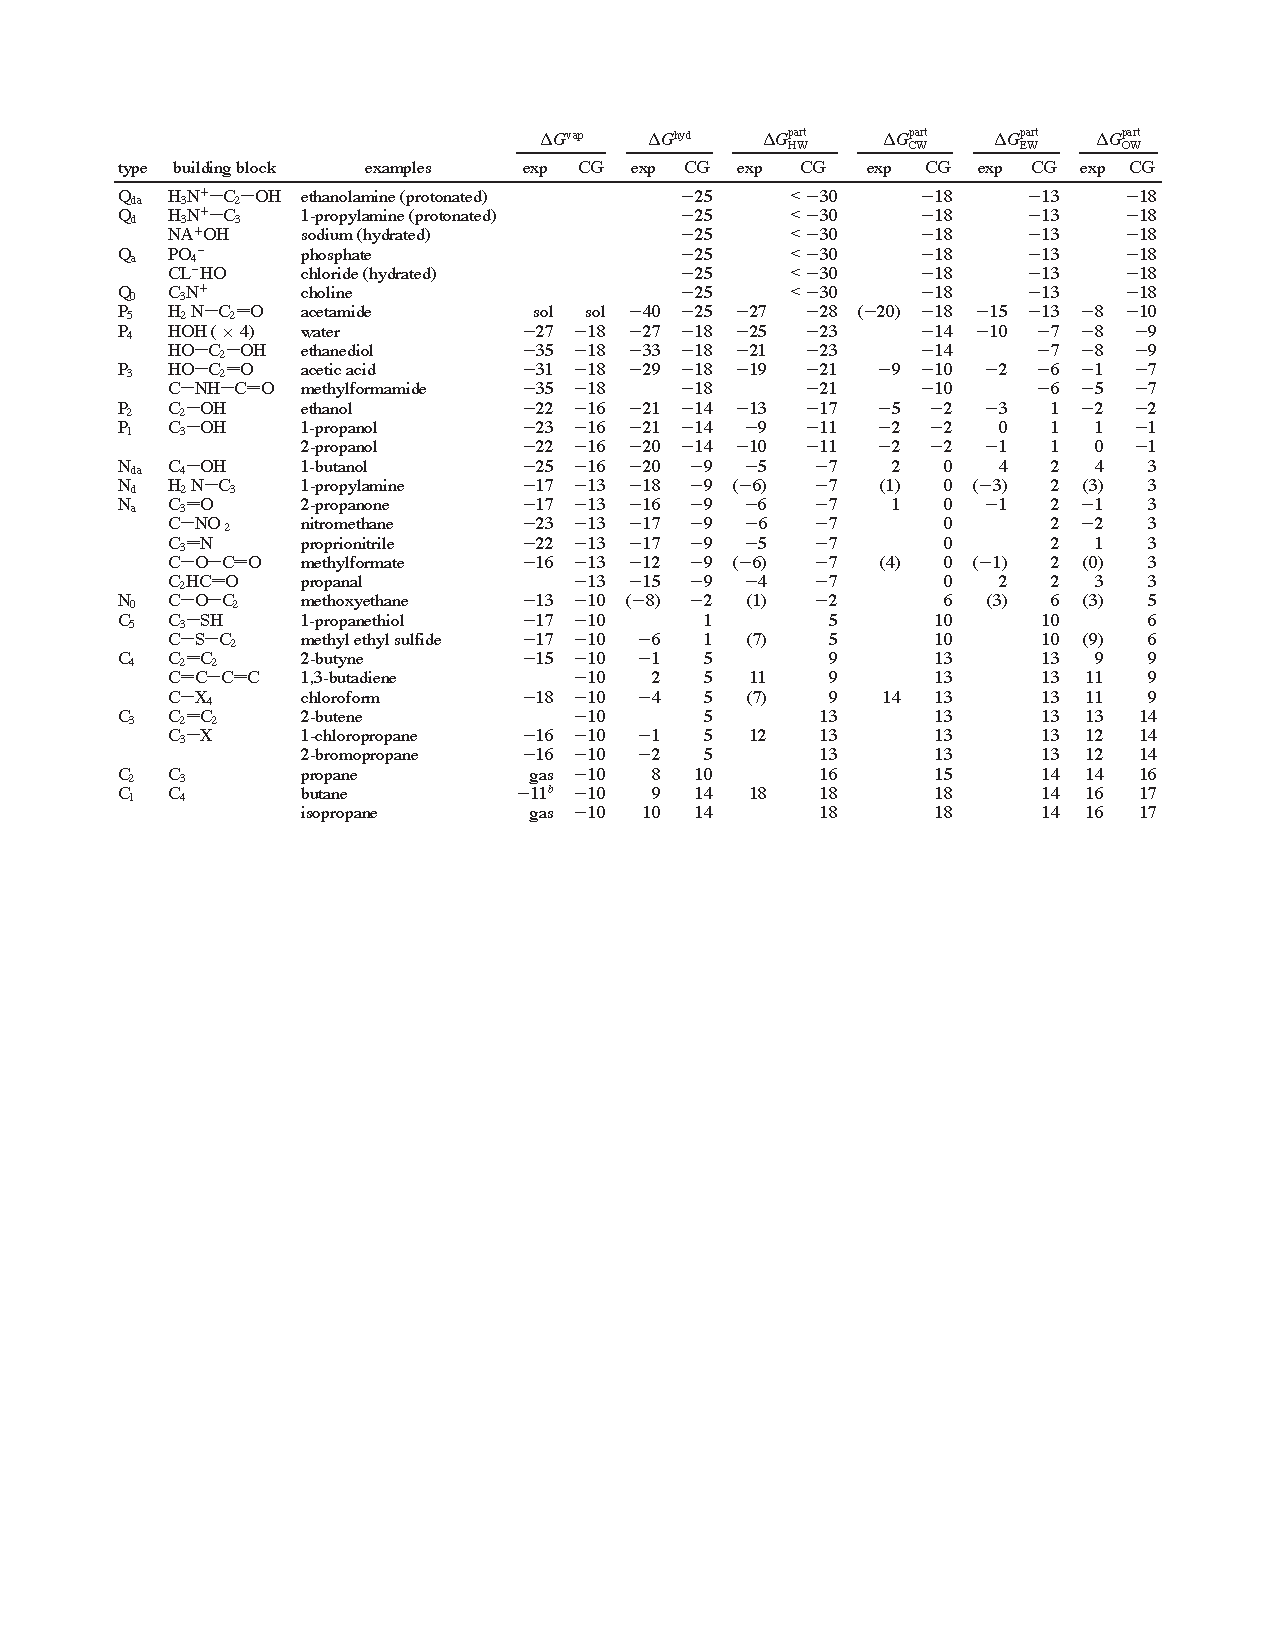
\includegraphics[width=\textwidth]{img/martiniTarget}%
	\caption{Results summary: free energies of vaporization $\Delta G^\text{vap}$, hydration $\Delta G^\text{hydr}$ and partitioning $\Delta G^\text{part}$ between water (W) and organic solvents (hexadecane (H), chloroform (C), ether (E) and octanol(O)) compared to experimental values. Experimental properties in parentheses are estimates obtained from comparison to similar compounds. The statistical accuracy of the free energies obtained from the simulations is $\pm 1$~kJ/mol. $^b$ The temperature for the experimental data is $273$~K. Taken from \cite{Martini}.}
	\label{fig:martiniTarget}
\end{figure}
% \begin{adjustwidth}{-3cm}{-5cm}%%
% 	\begin{minipage}[c]{1.4\textwidth}%
% 		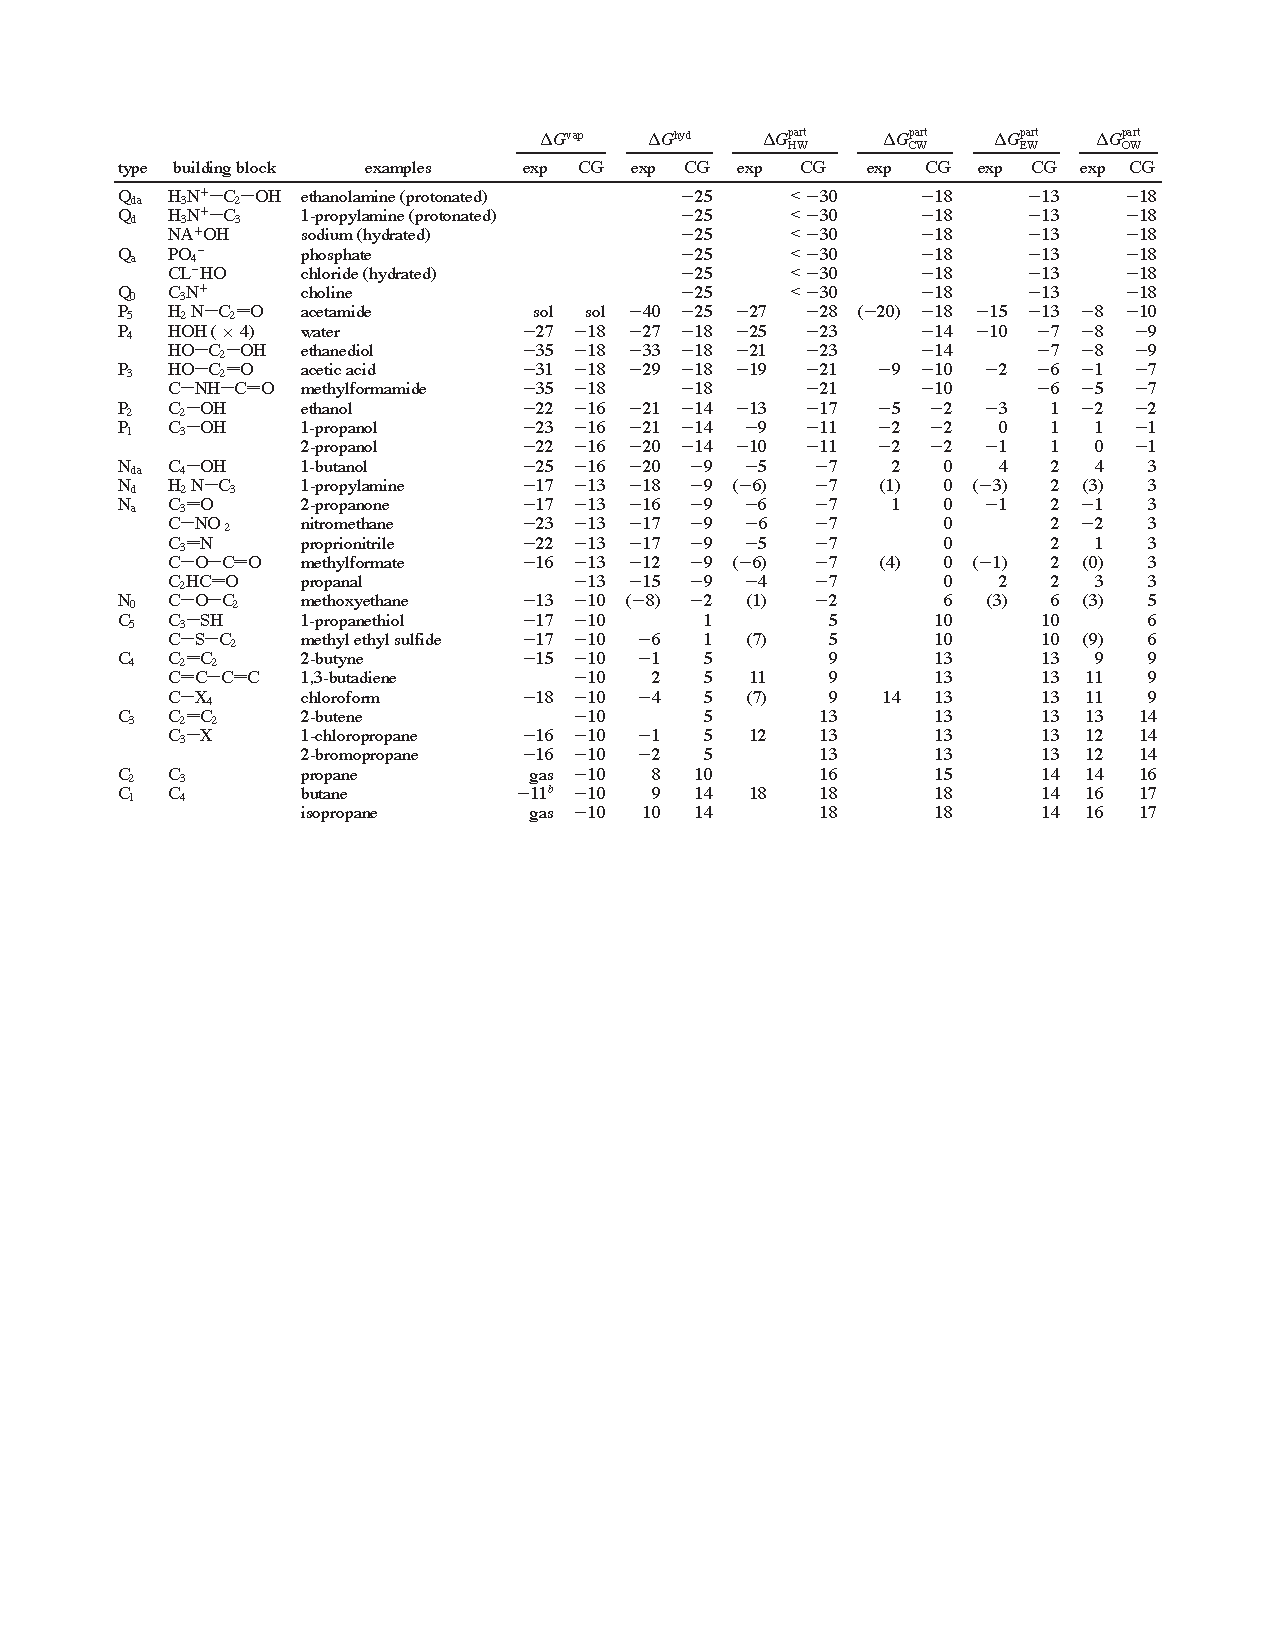
\includegraphics[width=\textwidth]{img/martiniTarget}%
% 		\captionof{figure}{Results summary: free energies of vaporization $\Delta G^\text{vap}$, hydration $\Delta G^\text{hydr}$ and partitioning $\Delta G^\text{part}$ between water (W) and organic solvents (hexadecane (H), chloroform (C), ether (E) and octanol(O)) compared to experimental values. Experimental properties in parentheses are estimates obtained from comparison to similar compounds. The statistical accuracy of the free energies obtained from the simulations is $\pm 1$~kJ/mol. $^b$ The temperature for the experimental data is $273$~K. Taken from \cite{Martini}.}
% 		\label{fig:martiniTarget}
% 	\end{minipage}
% \end{adjustwidth}

\subsection{Polarizable Water model}
\label{sec:pw}
Water play a crucial role in any biomolecular systems thus it is important to correctly describe its behavior. 
Since the \martini water model does not directly take into account the electrostatic interaction between water and the other molecules because it does not have any charge and it interact only via Van der Waals interaction, thus a simple implicit medium is used to take into account the main effects of water, screening and polarizability. However any biomolecular process involve charged species moving between regions of different dielectric constant. Due to the change in electrostatic screening between those environments, the strength of the interaction between the moving charges and the surrounding molecules also changes, but this effect can not be consider in an implicit medium model. Thus can have important consequences for the way biological activity is controlled. In order to capture the inhomogeneous nature of the dielectric response an explicit medium has to be used. 
\begin{figure}[!ht]
	\centering
	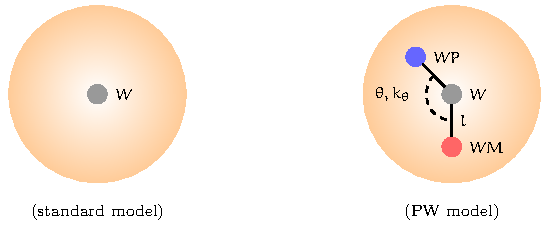
\includegraphics[width=0.8\textwidth]{./img/PWModel/PWModel}
	\caption{Schematic representation of the \acs{PW} bead. Shaded orange spheres correspond to the Van der Walls radii of the central neutral particle $W$. The blue particle is the positively charged while the red is the negatively charged.}
	\label{fig:PW}
\end{figure}

In the same fashion of the \martini philosophy, Yesylevskyy \etal\, \cite{PW} have developed a \acf{PW} model that better describe the real behavior of water. As before four water molecules is associated to one \ac{PW} bead. The new water bead actually consists of three particles instead of one in the standard \martini model. 
In figure~(\ref{fig:PW}) the topology of the \ac{PW} and a comparison between the old model is shown. The central particle $W$ is neutral and interacts with other particles in the system with only Lennard--Jones potential, just like the standard water bead thus as a $P_4$ \martini bead (see figure~(\ref{fig:martiniInteractions}) for the interactions matrix). There are two additional particles, namely $WP$ and $WM$, that are bound to the central particle and carry a positive and negative charge $|q| = 0.46\mathsf{e}$ respectively, where $\mathsf{e} = 1.60217653(14) \cdot 10^{-19}$~C is the unit electron charge. They interact with other particles in the system by the Coulomb interaction only. The bonds $W-WP$ and $W-WM$ are constrained to have a fixed distance $l = 0.14$~nm. 
The electrostatic interaction between $WP$ and $WM$ inside the same bead are exclude thus they are transparent toward each other and they can rotate around the $W$ particle. As a consequence the dipole momentum of the water bead depends on the relative angular position $\theta$ of $WP$ and $WM$: It can vary from zero ($\theta = 0$), to $2ql$ ($\theta = \pi$). A harmonic angle potential with equilibrium angle fixed to $\theta_0 = 0$ and a force constant $k_\theta = 4.2$~kJ/(mol$\cdot$rad$^2$) is added to control the rotation of $WP$ and $WM$ particles around the $W$ particle so to adjust the distribution of the dipole momentum. The value of the equilibrium angle is consistent with the fact that in an apolar medium the total dipole momentum of a water molecule is zero. 
Since in this model the screening and polarization effects are treated explicitly the global dielectric constant is then reduced from $\varepsilon_r = 15$, used in the standard \martini, to $\varepsilon_r = 2.5$. Moreover, since the \ac{PW} beads attract each other stronger then the standard water beads because of additional electrostatic interactions the strength $\epsilon_{WW}$ of the Lennard--Jones interaction between $W$ particles must be reduced. They found that change the Lennard--Jones strength from an $I$ level to an $III$ level can do the trick (see table~(\ref{tab:martiniEpsilon}) for the various interaction levels). While $\sigma$ remains set to $0.47$~nm.

The parametrization of $q$, $k_\theta$ and $\epsilon_{WW}$ are obtained, in addition to the basic target properties of the \martini \ac{FF}, also trying to reproduce the dielectric constant, density and dipole momentum of a pure water phase. For a more details about the parameterizations and testing methods the reader is addressed to the article by Yesylevskyy \etal\,\cite{PW}. An important question is the use of the \ac{PME} method to treat the long range electrostatic interaction. The authors found that, despite the loss of performance, in addition to the \ac{PW} model, the use of the \ac{PME} method contributes to a more realistic description of the processes involved in a biomolecular environments. In particular, some interesting results of utility for this thesis work, concern a better description of some properties of lipid membranes. One is the translocation of charged ions through a lipid bilayer that is described in a more realist detail: The authors found that the simulations with \ac{PW} and \ac{PME} are approaching the atomistic results better then the standard \martini \ac{FF}. Another important phenomenon about lipid membranes consist in the electroporation of membrane by \ac{PW} beads due to an electric field across the membrane (for example, created by a cross membrane ions imbalance) and, relented to this, the translocation of ions across the membrane helped by a so called ``\textit{water finger}'' a water defect inside the membrane that seems to be the trigger of the ions translocation. Such phenomenons are clearly evident in atomistic simulation however never occurred using the standard \martini \ac{FF} thus the importance to use the \ac{PW} model together with \ac{PME} method.
%Despite this the loss of performance is clearly related to the fact that \ac{PW} increase by a factor $\times 3$ the number of particles in the system related to water.

%\subsection{Applications}

\subsection{Limitations of MARTINI FF}
As we have seen in~\ref{sec:CGModel} the \ac{CG} \acp{FF} are computationally advantages, however a price has to be paid. Although the \martini \ac{FF} is still a finer \ac{CG} \ac{FF}, some limitations are shared with other \ac{CG} models at a fundamental level, such as the chemical and spatial resolution, which are both limited compared to atomistic models. One of the most important question is the \ac{DOF} reduction: This affects the entropy of the system which is underestimated and, as consequence of the \martini parameterizations, also the balance between enthalpy is not correct described. Since the \martini model is built with the constraint that the partitioning free energy $\Delta G = \Delta H - T\Delta S$ must be conserved with the atomistic case, together with an intrinsic loss of entropy, the enthalpic contribution must decrease with respect to the atomistic model\footnote{If a $NVT$ ensemble is used the correct potential is $\Delta A = \Delta U - T\Delta S$, thus the incorrect balance is between the internal energy and the entropy.}. Moreover this mean that the temperature dependence of a \ac{CG} model is a priori not correct, anyway this is not our case since we use only a $NVT$ or a $NPT$ ensemble with an external thermostat coupling.

Another consequence of \ac{CG} \acp{FF} is related to the \ac{PEF} that becomes smoother respect to the atomistic case. This effectively results in more sampling of the energy landscape in a given time period, speeding up the kinetics of the system and allowing the use of an higher time steps with longer simulation times. However the speed--up is not easily predictable and is not likely to be the same for different systems and maybe it is dependent on the type of molecule. Nevertheless for the \martini \ac{FF} an average scaling factor of $4$, based on lateral diffusion coefficients of lipids in membranes, is commonly used, of course with some care. Another smaller source of errors is due to the choice of masses: Since ensemble properties is not affected by particles mass, in order to increase the efficiency, all the \martini beads have the same mass of $72$~amu. This leads in some uncertainty in the dynamics of the system making the time scaling for different beads non--trivial.

A problem involving the Lennard--Jones potential as a model of Van der Waals interaction in \martini, is that the steep repulsion leads to an over--structuring of fluids compared to atomistic models. The direct and most evident implication is the melting point of the water that is $290 \pm 5$~K. A practical partial solution is the use of the so called ``anti--freeze'' particles named BP$_4$ type. The Lennard--Jones interaction between these particles and water is modified with a slightly larger Van der Waals radius parameter, $\sigma = 0.57$~nm and a stronger interaction to be a level $O$ (see table~(\ref{tab:martiniEpsilon}) for the interaction level). Marrink \etal\, suggest that a mole fraction of $n_{\text{af}} = 0.1$ is sufficient to prevent freezing without affecting the other properties of water. Some other properties of water are not accurate described such us the surface tension of air/water interface that leads in problem to water/oil interfaces formation. Using the \ac{PW} model these properties improve slightly. For a more comprehensive discussion about the limitations of the \martini \ac{FF} the reader is addressed to the review by Marrink \etal\, \cite{MartiniReview}.

\section{Advanced sampling methods}
The quantity of particular importance for the equilibrium statistical mechanics of which we are interested to obtain with \ac{MD} technique is the free energy function: the Gibbs free energy $G$ for the isobaric--isothermal ensemble and $A$ the Helmholtz free energy for the canonical ensemble. Being related to the partition function of an ensemble, the free energy is the generator through which other thermodynamic quantities are obtained via differentiation. However often we are particularly interested in the free energy difference between two thermodynamic states, instead of the absolute value. This because free energy differences are the driving force of any process and they tell us, for example, if a chemical reaction occurs spontaneously, whether a given solute is hydrophobic or hydrophilic, if a protein conformational change take place or whether some molecules in water solution are able to self--assembles into a more complex system and so forth. Moreover, often, we are interested also in the \ac{FES}: the free energy in function of some generalized coordinates, called \acp{CV} of the system. These small set of variables can describe, in a simple and useful manner, some chemical, thermodynamic or mechanical processes that take place in the system, for example, the free energy in function of the distance between the \ac{COM} of two molecules give us information about their attraction or repulsion and if they form a bound state; or in function of a rotational angle of a molecule bond to obtain all the possible stable configurations and so on. Thus the \ac{FES} provides a map of the stable conformations, the relative stability of these conformations and the barrier heights that must be crossed for the processes to take place. It is necessary to stress out that in many cases one do not know exactly \textit{a priori} the \ac{FES} about a certain process and so one want to know it also for understand if other minima energy configurations exist, in addition to those known, how stable they are and what are the energy barriers to go from one minima state to an other\footnote{Sometimes thought the cinematic of an \ac{MD} simulation one can gamble an estimate of the functional form of the \ac{FES}, looking for the relative probability to stay in a meta--stable state rather then the other. Clearly this means that both meta--stable states are to be sampled, as we shall see later it depends of the height of the energy barriers.}. 
Despite this, the calculation of free energy difference of two thermodynamic states (that leads an \textit{a priori} knowledge of the two stable states) and the calculation of the \ac{FES} are one of the main challenges in \ac{MD} simulations for biomolecular applications.

Lets us suppose that we are interested in the \ac{FES} of the \ac{CV} $s(\vec r)$ and we are working in a isobaric--isothermal ensemble with an isotropic system. Following section~\ref{sec:statmec}, the Gibbs free energy along the \ac{CV} is obtained as
\begin{equation}
	G(s) = -k_BT \ln Q(s)
	\label{eq:fes}
\end{equation}
where $Q(s)$ is the partition function with all other \ac{DOF} expect for $s(\vec r)$, integrated out. This leads as follow
\begin{equation*}
	Q(s) = \frac{1}{\mathcal{Z}_{NpT}} \int_0^{+\infty}\ dV \ \int_\Omega e^{-\beta(\mathcal{H}(\vec x) + pV)}\delta(s(\vec r) - S)\ dx
\end{equation*}
since $s(\vec r)$ do not depends on particles momenta, from equations~\eqref{eq:hamiltonian} and~\eqref{eq:nptPartition}, it can be rewritten as
\begin{equation}
	Q(s) =  \frac{ \int_\Omega e^{-\beta U(\vec r)}\delta(s(\vec r) - s)\ dr }{\int_\Omega e^{-\beta U(\vec r)}\ dr}
	\label{eq:CVprobability}
\end{equation}
where $U(\vec r)$ is the \ac{PEF}. $Q(s)ds$ can be interpreted as the probability of finding the system with $s(\vec x)$ between $s$ and $s + ds$. Since this equation contains a direct phase space integration can be rewritten in a more useful manner using the ensemble averages then, using the ergodic theorem in equation~\eqref{eq:ergotic}, as a time averages:
\begin{equation}
	Q(s) = \ave{\delta(s(\vec r) - s)} = \lim_{t\to +\infty}\frac{1}{\tau}\int_0^\tau \delta(s(\vec r(t)) - s)\ dt
	\label{eq:CVprobabilityAve}
\end{equation}

\ac{MD} simulations give us the possibility to sample a given ensemble via computational methods, in principle, in order to calculate the integrals in equation~\eqref{eq:CVprobabilityAve}. Unfortunately, since the time can not be infinity, the main problem related to \ac{MD} simulations is whether we are able to correctly sample \textit{all} the phase space of an ensemble in order to compute the ensemble average. Clearly the answer depends on the system in exam, if it is really simple maybe we can do that, otherwise probably no or it takes too time and/or we are not able to collect sufficiently data. This sampling problem can be summarized as follow: Regions in phase space around a local minimum of the \ac{PEF} (then a local minimum even in the \ac{FES}) are typically sampled well, whereas regions of higher energy are sampled rarely. Despite they leads with a small contribution to the partition function, due to Boltzmann factor, a bigger challenge, related to overcome regions of higher energy, is to sample other minima of the \ac{PEF}, that can be of lower or same energy and instead can leads to a important contribution to the ensemble averages. This is the \textit{rare events problem}. When the system is moving in the \ac{PEF} landscape the only way to escape from a local minimum is due to thermal fluctuations and so energy barriers that are higher then $\sim k_B T$ have a small probability of being overcame. Then the sampling problem! Moreover the energy landscape, even for a small molecule, it is extremely wrinkled and the large number of free energy minima is far more than can be sampled in a typical \ac{MD} simulation. Thus the principal reason for the use of the just introduced \acp{CV}, they can limit the sampling necessity to those regions of phase space that are most important to the process under study, hoping that, as the \ac{DOF} reduction in a \ac{CG} \ac{FF}, the limited sampled regions are sufficient to correctly describe the process.

Several methods are developed and are still in development in order to solve the just described sampling problem. This method are all based on advanced sampling techniques that allow us to
\begin{itemize}
	\item Escape from a local energy minima, in order to explore other regions of the phase space;
	\item Calculate free energy difference between two thermodynamic states;
	\item Compute the \ac{FES} along one or a small set of \acp{CV};
	\item Try to capture and study the transition state of a process (in function of some \acp{CV}).
\end{itemize}
The common basic idea is to introduce additional \ac{DOF} along the \acp{CV} in order to modify or add some potential energy, to the \ac{PEF} that drive the system from one state to another. This additional potential is called \textit{biased potential} and those advanced sampling methods are grouped in the so called \textit{biased} \ac{MD} to distinguish from the \textit{un--biased} \ac{MD} in which the system is not driven. In particular we describe only those methods used in this thesis work: \textit{Umbrella sampling method} and \textit{Metadynamics}. For a more comprehensive discussion the reader is addressed to the review by Kästner \cite{Umbrella} for the former and to the review by Laio and Gervasio \cite{MetadReview} for the latter. Moreover in the books of Tuckerman \cite{Tuckerman} other methods are described.

%It is clear, from the previous sections, that if we are able to correctly sample an ensemble, the law of statistical mechanics (\ref{sec:stamec}) leads the way to obtain thermodynamic properties and macroscopic observables of a system that is part of the ensemble; while \ac{MD} simulations (\ref{sec:MD}) give us the possibility to sample a given ensemble via computational methods. Unfortunately the main problem related to \ac{MD} simulations is whether we are really able to correctly sample \textit{all} the phase space of an ensemble. Clearly the answer depends on the system in exam, if it is really simple maybe we can do that, otherwise probably no or it takes too time and/or we are not able to collect sufficiently data. Let us to focus more in detail about the problem.

\subsection{Umbrella sampling}
Umbrella sampling method was developed by Torrie and Valleau and today is one of the most mature and broadly accepted method for calculating free energy differences. The basic idea is to drive the system from a known state $A$ to an other known state $B$ through a deterministic path defined on the \ac{CV} $s(\vec r)$ chosen to describe the process. This methods is well suitable for one \ac{CV} otherwise the computational performance degrades rapidly with the number of \acp{CV}. The idea is to divide the path into a discrete number of segment $N_w$ and take a subset $\{s_i\}$ of the values assumed by the continuos \ac{CV} from state $A$ to $B$ along the path. For each of those target values $s_i$ a bias potential $w_i(s)$ depending only on $s$ is added to \ac{PEF} in order to restrain the system to the target value. Then \ac{MD} simulations are performed for each value. Those $N_w$ independent simulations are commonly called \textit{windows} for which the \ac{CV} assume different values. Then, with an analysis method, all data collected with the windows are combined together to compute the \ac{FES} along the chosen \ac{CV}. In figure~(\ref{fig:umbrellaPath}) an example of the windows selection is shown.
\begin{SCfigure}
	\centering
	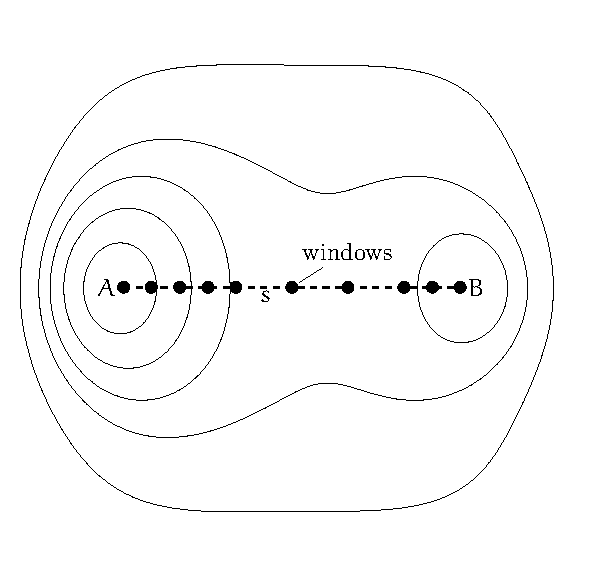
\includegraphics[width=0.6\textwidth]{./img/umbrellaPath/umbrellaPath.pdf}
	\caption{Example of an umbrella sampling windows selection. The contour plot represent a $2$--minima free energy profile through which the system is evolved. The dashed line is the path along the \acs{CV} $s(\vec r)$ that connect state $A$ to $B$. The black filled circles represent the selected windows for different values of $s$.}
	\label{fig:umbrellaPath}
\end{SCfigure}

Suppose $w_i(s)$ to be the bias potential applied on window $i$ in function of the \ac{CV} $s(\vec r)$. Then the biased \ac{PEF} of window $i$ become $U_i^b(\vec r) = U(\vec r) + w_i(s)$; where the superscript $b$ denotes biased quantities. With the substitution $U(\vec r) \rightarrow U_i^b(\vec r)$ in equation~\eqref{eq:CVprobability} the corresponding biased partition function integrated over all \ac{DOF} but $s$ and exploiting the Dirac delta properties, yields to
\begin{equation*}
	Q_i^b(s) = e^{\beta w_i(s)}\frac{ \int_\Omega e^{-\beta U(\vec r)}\delta(s(\vec r) - s)\ dr }{\int_\Omega e^{-\beta (U(\vec r) + w_i(s(\vec r)))}\ dr}
\end{equation*}
In order to use equation~\eqref{eq:fes} to obtain the \ac{FES}, we need to recover the un--biased partition faction $Q_i(s)$ like in equation~\eqref{eq:CVprobability}. This can be done (see \cite{Umbrella}), obtaining the following expression
\begin{equation}
	\begin{aligned}
	Q_i(s) &= Q_i^b(s) e^{\beta w_i(s)}\ \frac{ \int_\Omega e^{-\beta U(\vec r)}e^{-\beta w_i(s(\vec r))}\ dr }{\int_\Omega e^{-\beta U(\vec r)}\ dr} = \\
		   &= Q_i^b(s) e^{\beta w_i(s)}\ \ave{e^{-\beta w_i(s)}}
	\end{aligned}
	\label{eq:windowPartFunc}
\end{equation}
then the \ac{FES} for window $i$ is obtained simply by equation~\eqref{eq:fes}
\begin{equation*}
	G_i(s) = -k_BT \ln Q_i^b(s) - w_i(s) + C_i
\end{equation*}
where $Q_i^b(s)$ is obtain as an ensemble average via the biased \ac{MD} simulation like equation~\eqref{eq:CVprobabilityAve} and $w_i(s)$ is a known function. $C_i$ is an addictive constant independent of $s$ that connect the free energy curves $G_i(s)$ of different windows. As we shall see, in order to combine more windows to calculate a global \ac{FES}, all set $\{C_i\}$ must be computed.

\paragraph{\textbf{Weighted histogram analysis method}} Different analysis methods have been developed in order combine informations collected from the $N_w$ windows. The aim of those methods is to compute the global un--biased partition function $Q(s)$ from the set of biased partition function $\{Q_i(s)\}$ in order to extract the global \ac{FES} $G(s)$. The most commonly used method is the \ac{WHAM} \cite{WHAM}, \cite{gWHAM}. The philosophy behind is to minimize the statistical error in the calculation of $Q(s)$. For each of the $N_w$ biased windows a set of histograms $\{h_i(s)\}$ with $n_i$ bins, representing the set $\{Q_i(s)\}$, is recorded. The global distribution function is computed as follow
\begin{equation}
	Q(s) = \sum_{i=0}^{N_w} p_i h_i(s), \qquad \sum_{i=0}^{N_w} p_i = 1
	\label{eq:whan1}
\end{equation}
where $p_i$ are weights chosen to minimize statistical error on $Q(s)$. Those leads to
\begin{equation}
	p_i = \frac{n_ie^{-\beta (w_i(s) - C_i)}}{\sum_{j=0}^{N_w} n_je^{-\beta (w_j(s) - C_j)}}
	\label{eq:whanwheight}
\end{equation}
where $n_i$ is the total number of independent bins in the $i-$th histogram. The problem now is to compute the set of constants $\{C_i\}$. We can not use the integrals in equation~\eqref{eq:windowPartFunc} for the problems already described at the begging of this section, but the second line give us an idea. The ensemble average can be computed using the global distribution function $Q(s)$ as follow
\begin{equation}
	e^{-\beta C_i} = \ave{e^{-\beta w_i(s)}} = \int Q(s) e^{-\beta w_i(s)}\ ds
	\label{eq:whan2}
\end{equation} 
Because $Q(s)$ in equation~\eqref{eq:whan1} depends on the set of constants $\{C_i\}$ and \textit{vice versa}, both equations must be solved in a iterative self--consistent manner. A first guess of set $\{C_i\}$ is used to compute the weights from equation~\eqref{eq:whanwheight} then from equation~\eqref{eq:whan1} $Q(s)$ is computed and it is used to obtain a new set of constants $\{C_i\}$ from equation~\eqref{eq:whan2} and so on until both equations are satisfied. When the iteration procedure is completed the global \ac{FES} $G(s)$ is obtained from equation~\eqref{eq:fes}. One important consideration about \ac{WHAM} is that each window must be sufficient overlap between the distribution of the chosen value of the \ac{CV} otherwise the statistical error due to the combining procedure can be too high or the iterative producer itself can lead to convergence problem. In general a set of windows are performed then if they are not sufficient other windows are carry out.

\paragraph{\textbf{Bias potential}} The bias potential is chosen such that sampling along the \ac{CV} is uniform. Obviously $w(s) = -G(s)$ is the best optimal choice, unfortunately $G(s)$ is not \textit{a priori} known. Together with \ac{WHAM} a simple harmonic bias potential is most commonly used for its simplicity. In order to restrain the system to the target value $s_i$ of the \ac{CV} $s(\vec r)$ along the path chosen to connect state $A$ and $B$, each window is biased with a harmonic potential of the form
\begin{equation*}
	w_i(s) = \frac{1}{2}K (s - s_i)^2
\end{equation*}
The choice of $K$, the strength of the bias potential, is a critical point. $K$ has to be large enough to drive the system over the barrier. However too large $K$ cause too narrow distribution that can cause overlap problems, thus the necessity for $K$ to be as small as possible to allow for much overlap between windows.

%\paragraph{\textbf{error estimation}}

\bigskip The implementation of the umbrella sampling method can be summarized in the following procedure
\begin{itemize}
	\item A \ac{CV} that well describe the transition process from state $A$ to $B$ and a connecting path are chosen;
	\item A subset of the values assumed by the \ac{CV} along the path are taken and for each a biased \ac{MD} simulation is performed (windows)\footnote{Since each biased simulation is independent they can be performed in parallel with the other.};
	\item Using \ac{WHAM} the set of biased partition functions $\{Q_i(s)\}$ are combined in order to compute the global partition function $Q(s)$. Then $G(s)$ is calculated;
	\item If the biased partition functions are not well overlapping then more windows have to be performed.
\end{itemize}

 
\subsection{Metadynamics}
The metadynamics method was originally developed by Parrinello and Laio \cite{MetadParrinello} with the first aim to accelerate the escaping from a free energy minima in order to explore other phase space regions. Soon the success of the methods leads a creation of an unified framework for computing free energies in function of few \acp{CV} and accelerating rare events. The main advantages respect to umbrella sampling method is that several \acp{CV}, instead of only one, can be simultaneously used without affecting the simulation performance. The basic idea of the metadynamics is to enhance the dynamics of a system along some \acp{CV} simply by filling the corresponding energy minimum which an history--dependent bias potential, in order to samples a larger and larger portion of the phase space. If the deposited energy is sufficient the system is favorably disposed to overcome the energy barrier to go to another meta--stable state. This novel idea is moreover supported by the assumption of Parrinello and Laio, based on experimental and heuristic results, that iteratively summing the deposited potential during the biased \ac{MD} simulation leads to an estimator of the \ac{FES} along the chosen \acp{CV} in the region explored. If $\vec s(\vec r) = (s_1(\vec r), \cdots, s_n(\vec r))$ is the \acp{CV} vector, where $n$ is a small number, and $w(\vec s, t)$ is the bias potential deposited every $\tau$ \ac{MD} time steps the ``metadynamics'' history--dependent potential acting on the system at a time $t$ is given by
\begin{equation*}
	w_M(\vec s, t) = \sum_{\substack{i=0 \\ i\tau < t}} w(\vec s, i\tau)
\end{equation*}
where $t$ is the time in unit of \ac{MD} time step. The time dependence in the bias potential $w(\vec s, t)$ is needed since it have to depend on the values assumed by the \acp{CV} at some previous \ac{MD} steps. The Parrinello and Laio assumption yields to the following expression
\begin{equation}
	\lim_{t\to + \infty} w_M(\vec s, t)  \simeq -G(\vec s) + C
	\label{eq:metadfes}
\end{equation} 
where $C$ is an addictive constant. Since the history--dependent potential iteratively compensates the underlying \ac{FES}, the system evolved with metadynamics \textit{tends to escape from any energy minima via the lowest saddle point}. Thus, to the contrary of umbrella sampling metadynamics is suitable, not only to compute efficiently \ac{FES}, but also to explore new reaction path and accelerate the observation of rare events. If the \acp{CV} are chosen sensibly the system will quickly find its way over the lowest free energy saddle point and evolve over the next minimum as it would do in a \textit{very long} \ac{MD} simulation.

An intrigued bias potential can be deduced considering equation~\eqref{eq:CVprobabilityAve}. The Dirac delta function can be expressed by an its approximant:  
\begin{equation*}
	\delta(x-a) = \lim_{\sigma\to 0}\ \frac{1}{\sqrt{2 \pi \sigma^2}}e^{-(x-a)^2/(2\sigma^2)}
\end{equation*}
then substituting in equation~\eqref{eq:CVprobabilityAve} we have
\begin{equation*}
	Q(s) = \frac{1}{\sqrt{2\pi}}\lim_{t\to +\infty}\ \lim_{\sigma\to 0} \frac{1}{\sigma t}\int_0^t \exp{ \left ( -\frac{(s(\vec r(\tau))-s)^2}{2\sigma^2} \right )} \ d\tau
\end{equation*}
the equation above suggest as a component of the history--dependent bias potential the use of a Gaussian function centered around the values assumed by the \acp{CV} at a time $t$. Then the bias potential component, extended to a multiple \acp{CV}, is chosen as follow
\begin{equation*}
	w(\vec s, t) = w\ \exp\left ({-\sum_{i=0}^n \frac{(s_i - s_i(\vec r(t)))^2}{2{\delta s_i}^2} }\right )
\end{equation*}
where $w$ is the height and $\delta s_i$ is the width of the deposited Gaussians.

For setting up a metadynamics simulation, then there are three parameters to carefully choose: the height $w$ and the width $\delta s_i$ of the deposited Gaussian and the stride of deposition $\tau$. All these parameters affect the accuracy and the efficiency of the free energy profile reconstruction. Clearly if the Gaussians are big and large or placed quickly the \ac{FES} will be explored at a fast pace but the reconstructed profile will be affected by large errors. Instead if they are small or placed infrequently the reconstruction will be accurate but will take a longer time. Moreover the time required to escape from a local minimum is determined by the number of Gaussians necessary to fill the well. This number is proportional to $(1/\delta s)^n$ \cite{MetadReview}, then the necessity to maintain the number $n$ of \acp{CV} as small as possible or increase the Gaussian width. On the other hand the history--dependent potential can only reproduce features of the \ac{FES} on a scale larger then $\sim \delta s$. Small criteria can be used to choose the $\delta s$ and $\tau$ parameters; the former by monitoring the standard deviation of the \acp{CV} in an unbiased \ac{MD} simulation and the latter by considering the relaxation time of the system after a Gaussian is deposited: clearly the bigger is the Gaussian the more time is needed by the system to well relax. However does not exist an universal and general recipe to choose these parameters, only some knowledge of the system and process under study can revel the right way; they can certainly fine tuned in successive steps.

In figure~(\ref{fig:metadEs}) an example of the time evolution of a metadynamics simulation is shown. We can see that as the deposited Gaussians increases the system is able to visit more regions of the phase space. Moreover as the simulation time increases, when the energy landscape (lower panel) become flat the system become diffusive (upper panel) on the whole energy profile. Thus we can stop the metadynamics simulation obtaining the right \ac{FES} less then a constant as in equation~\eqref{eq:metadfes}. 
\begin{SCfigure}
	\centering
	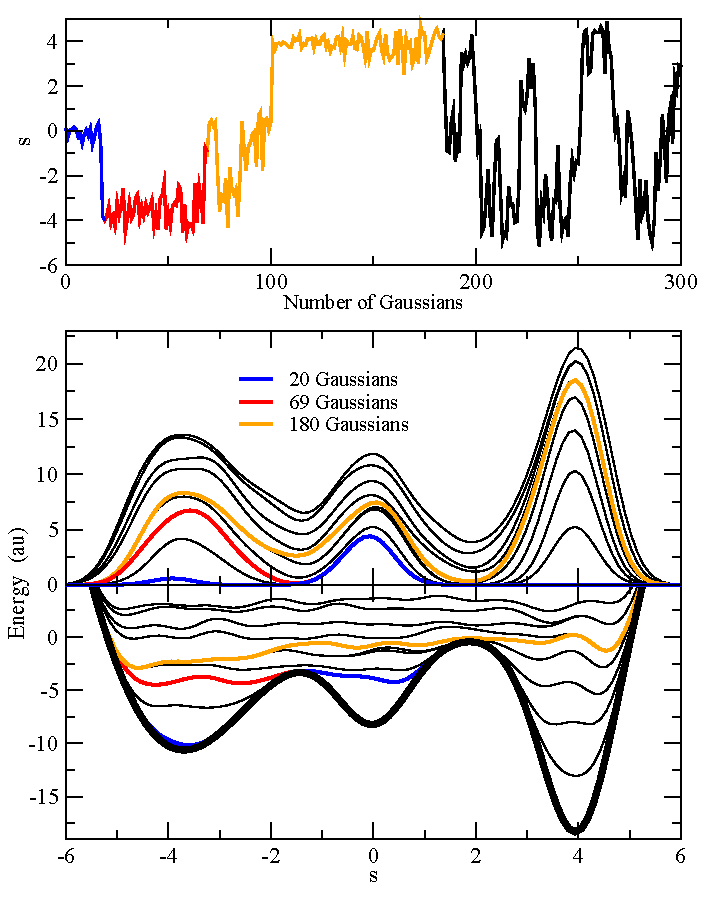
\includegraphics[width=0.55\textwidth]{./img/metadEs}
	\caption{Example of a time evolution of a metadynamics simulation. Top: time evolution of the \acs{CV} of a system evolved on the 3--minima \acs{FES} represented by the black thick line in the lower panel. Middle: time evolution of $w_M$ the history--dependent bias potential i.e. minus the \acs{FES}. Blue line: $w_M$ as when the first minimum is filled and the system escapes to the second minimum; red line: as when also the second minimum is filled; orange line: when the entire profile is filled and the dynamics becomes diffusive on the whole energy landscape. Lower panel: time evolution of the sum of $w_M$ (same color scheme). Taken from \cite{MetadReview}.}
	\label{fig:metadEs}
\end{SCfigure}

Keeping in mind figure~(\ref{fig:metadEs}) a summary of the behavior of metadynamics and the validity of equation~\eqref{eq:metadfes} can be qualitatively understood in the limit of slow deposition. This means that $w_M(\vec s, t)$ varies slowly and the probability to observe $\vec s$ is approximately proportional to the Boltzmann factor $e^{-\beta(G(\vec s) - w_M(\vec s, t))}$. If the function in the exponential has some local minimum due to $G(\vec s)$, $\vec s$ will preferentially be localized in the neighborhood of this minimum and an increasing number of Gaussians have to be added until it is completely filled. When the minimum is filled the system reach the condition $G(\vec s) \sim w_M(\vec s, t)$ and the probability distribution would be approximately flat and we can say that the system become diffusive in the region explored by the simulation. Then, in this regions, the location of new Gaussians is no more affected by the difference between $G(\vec s)$ and $w_M(\vec s, t)$ and they are deposited randomly over the flat free energy profile. Hence the \acp{FES} reconstructed after that point, as visible in figure~(\ref{fig:metadEs}), are affected by some corrugations, due to newly deposited Gaussians, of the order of $w$. From that point it says that the metadynamics has reached the \textit{convergence} in the sampled region: the \ac{FES}, as the Gaussians deposition increase, do not change its shape but it is only shifted downward along the energy axes.

\paragraph{\textbf{convergence}} As just explained before, the convergence of the metadynamics in a specific region of the \acp{CV} space is reached when the system become diffusive in this region, i.e. when the \acp{CV} can assume all possible values compatible to the sampled region. This is a crucial point for the metadynamics method in order to obtain the best possible estimator of the \ac{FES}, in the sampled region. Clearly, in order to save computational time, if one want only to give the possibility to the system to escape from an energy minimum is not necessary to reach the convergence otherwise it is an important point. Unfortunately in most system is not trivial to identify precisely when the diffusive regime has reached. In most cases a practical method to assess the convergence of metadynamics simulations is based on monitoring the free energy difference between two reference point: when the difference is approximately flat then the convergence should be reached.

\paragraph{\textbf{error estimation}} After the proper convergence is reached the error on the \ac{FES} estimator is clearly dependent on the chosen parameters. The best way to estimate the statistical error introduced by the metadynamics is to perform several statistically independent metadynamics runs. Clearly the arithmetic average of all the history--dependent potentials taken at the same time, after the convergence is reached, is still equal to the \ac{FES}. The statistical error of the \ac{FES} of a run can be considered as the standard deviation between the history--dependent potential $w_M(s,t)$ of that run and the averaged \ac{FES} $G(\vec s) \sim - \overline{w_M(\vec s,t)}$ and average it over the whole \acp{CV} space, as follow
\begin{equation*}
\overline{\epsilon}^2 = \frac{1}{\Omega_s} \int_{\Omega_s}  \overline{(w_M(\vec s,t) - \overline{w_M(\vec s,t)})^2}\ ds
\end{equation*}
where $\Omega_s$ is the whole \acp{CV} space. Laio \etal\, in \cite{MetadError}, by performing extensive numerical simulations of a Langevin stochastic system, have derived an approximate expression for the error estimator in function of the system and metadynamics parameters, as follow
\begin{equation*}
	\overline{\epsilon}^2 \propto \frac{LT}{D}\frac{w}{\tau} \delta s 
\end{equation*}
where $L$ is the size of the simulation box, $D$ is the system diffusion coefficient and $T$ is the system temperature. Since $\delta s$ is approximately fixed by the fluctuation of the \acp{CV} in a unbiased \ac{MD} run and/or by the granularity to be achieved in the \ac{FES} estimator, the error is dominated by the ration $w/\tau$. Thus a fine tuning of the Gaussians height and deposition pace is often needed in order to minimize the statistical error. Despite this, is commonly accepted to follow a procedure for the \ac{FES} and error estimators:
\begin{itemize}
	\item Several statistically independent metadynamics simulations are performed;
	\item After the convergence is reached for each run, the estimator of the \ac{FES} is the arithmetic average of the \ac{FES} obtained from equation~\eqref{eq:fes} for each simulations (each free energy profile appropriately normalized);
	\item The statistical error on the averaged \ac{FES} is performed considering its standard deviation. 
\end{itemize}
Alternatively one can perform a very long metadynamics run in which, for example, the system is diffusive for half simulation. Then one can chose as statistically independent history--dependent potentials some of them computed at different times in the diffusive region and follow the above procedure from the second point. Clearly one have to be careful about the decorrelation time between the chosen profiles, otherwise they are not statistically independent due the continuos nature of the metadynamics algorithm.

\paragraph{\textbf{performance optimization}} In general the computational overhead of adding metadynamics to an \ac{MD} simulation is usually not excessive, even if it depends on the implemented algorithms. However as the deposited Gaussians increases, each \ac{MD} step a larger and larger number of exponential terms have to be computed and summed in order to calculate the derivative of the history--dependent potential, i.e. the forces due to the metadynamics. Thus if the Gaussians are big or frequently deposited or the system takes a lot of time to reach the convergence, the computational overhead scales as the number of the deposited Gaussians. This can clearly leads to a lose of performance as the simulation time increase. A simple solution is to implement a discrete mesh grid on the \acp{CV} space in which the history--dependent potential is spread and stored into. When a new Gaussian is added the potential is updated in the whole grid. While, at each \ac{MD} step, in order to compute the derivative, the potential in a non--grid point is only estimated from an interpolation of some neighbor grid points. By this trick the computational overhead remains approximately constant as the simulation time increase.

\subsection{Umbrella sampling and metadynamics remarks}
Despite metadynamics is relatively recent while umbrella sampling is a well known and optimized method the former is steadily spread in the computational community against the latter. The most relevant reasons are its simplicity of implementation and the direct way to control efficiency and performance by changing the parameters of the Gaussians entering in the history--dependent potential. This gives to the metadynamics the possibility, with only one framework, to overcome different situations such as passing continuously from a fast and coarse exploration of the energy landscape to an accurate evaluation of the free energy profile, predict new stable configurations and structures, new reaction pathways, calculate free energy profiles and free energy differences.

In umbrella sampling the reconstruction of the free energy profile follow a predefined scheme designed for covering the chosen \acp{CV} space. In contract a well implemented metadynamics reconstruct efficiently the free energy profile. Starting from the current minimum and explore a larger and larger region of the accessible phase space dwelling on the low energy regions, which are statistically the most relevant, avoiding spend to much time in the irrelevant regions, the \ac{FES} is recursively reconstruct. Moreover which the advantage that each point in the \acp{CV} space is explored several times during the simulation. However a careful choice of the \acp{CV} is needed otherwise the history--dependent potential (and the reconstructed \ac{FES}) can evolves in an unpredictable manner.   

In a recent work by Davide Bochicchio \etal\, \cite{metaUSComparison} both methods for the \ac{FES} estimation included the error estimation, performance and accuracy are extensively compared with \ac{MD} simulations involving the transfer of a hydrophobic oligomers from water phase to hydrophobic core of a lipid membrane. The authors consider both at atomistic and \ac{CG} levels (\martini \ac{FF}). The authors found that, if the \acp{CV} are properly chosen and the parameters for the metadynamics are carefully tuned, the energy profiles reconstructed are reasonable identical between umbrella sampling and metadynamics, but the latter yields the same accuracy in a less time consuming simulation.  


%Manuale GROMACS 3.17.5 PP/PME ranks